% Options for packages loaded elsewhere
\PassOptionsToPackage{unicode}{hyperref}
\PassOptionsToPackage{hyphens}{url}
%
\documentclass[
]{book}
\usepackage{amsmath,amssymb}
\usepackage{lmodern}
\usepackage{iftex}
\ifPDFTeX
  \usepackage[T1]{fontenc}
  \usepackage[utf8]{inputenc}
  \usepackage{textcomp} % provide euro and other symbols
\else % if luatex or xetex
  \usepackage{unicode-math}
  \defaultfontfeatures{Scale=MatchLowercase}
  \defaultfontfeatures[\rmfamily]{Ligatures=TeX,Scale=1}
\fi
% Use upquote if available, for straight quotes in verbatim environments
\IfFileExists{upquote.sty}{\usepackage{upquote}}{}
\IfFileExists{microtype.sty}{% use microtype if available
  \usepackage[]{microtype}
  \UseMicrotypeSet[protrusion]{basicmath} % disable protrusion for tt fonts
}{}
\makeatletter
\@ifundefined{KOMAClassName}{% if non-KOMA class
  \IfFileExists{parskip.sty}{%
    \usepackage{parskip}
  }{% else
    \setlength{\parindent}{0pt}
    \setlength{\parskip}{6pt plus 2pt minus 1pt}}
}{% if KOMA class
  \KOMAoptions{parskip=half}}
\makeatother
\usepackage{xcolor}
\usepackage{color}
\usepackage{fancyvrb}
\newcommand{\VerbBar}{|}
\newcommand{\VERB}{\Verb[commandchars=\\\{\}]}
\DefineVerbatimEnvironment{Highlighting}{Verbatim}{commandchars=\\\{\}}
% Add ',fontsize=\small' for more characters per line
\usepackage{framed}
\definecolor{shadecolor}{RGB}{248,248,248}
\newenvironment{Shaded}{\begin{snugshade}}{\end{snugshade}}
\newcommand{\AlertTok}[1]{\textcolor[rgb]{0.94,0.16,0.16}{#1}}
\newcommand{\AnnotationTok}[1]{\textcolor[rgb]{0.56,0.35,0.01}{\textbf{\textit{#1}}}}
\newcommand{\AttributeTok}[1]{\textcolor[rgb]{0.77,0.63,0.00}{#1}}
\newcommand{\BaseNTok}[1]{\textcolor[rgb]{0.00,0.00,0.81}{#1}}
\newcommand{\BuiltInTok}[1]{#1}
\newcommand{\CharTok}[1]{\textcolor[rgb]{0.31,0.60,0.02}{#1}}
\newcommand{\CommentTok}[1]{\textcolor[rgb]{0.56,0.35,0.01}{\textit{#1}}}
\newcommand{\CommentVarTok}[1]{\textcolor[rgb]{0.56,0.35,0.01}{\textbf{\textit{#1}}}}
\newcommand{\ConstantTok}[1]{\textcolor[rgb]{0.00,0.00,0.00}{#1}}
\newcommand{\ControlFlowTok}[1]{\textcolor[rgb]{0.13,0.29,0.53}{\textbf{#1}}}
\newcommand{\DataTypeTok}[1]{\textcolor[rgb]{0.13,0.29,0.53}{#1}}
\newcommand{\DecValTok}[1]{\textcolor[rgb]{0.00,0.00,0.81}{#1}}
\newcommand{\DocumentationTok}[1]{\textcolor[rgb]{0.56,0.35,0.01}{\textbf{\textit{#1}}}}
\newcommand{\ErrorTok}[1]{\textcolor[rgb]{0.64,0.00,0.00}{\textbf{#1}}}
\newcommand{\ExtensionTok}[1]{#1}
\newcommand{\FloatTok}[1]{\textcolor[rgb]{0.00,0.00,0.81}{#1}}
\newcommand{\FunctionTok}[1]{\textcolor[rgb]{0.00,0.00,0.00}{#1}}
\newcommand{\ImportTok}[1]{#1}
\newcommand{\InformationTok}[1]{\textcolor[rgb]{0.56,0.35,0.01}{\textbf{\textit{#1}}}}
\newcommand{\KeywordTok}[1]{\textcolor[rgb]{0.13,0.29,0.53}{\textbf{#1}}}
\newcommand{\NormalTok}[1]{#1}
\newcommand{\OperatorTok}[1]{\textcolor[rgb]{0.81,0.36,0.00}{\textbf{#1}}}
\newcommand{\OtherTok}[1]{\textcolor[rgb]{0.56,0.35,0.01}{#1}}
\newcommand{\PreprocessorTok}[1]{\textcolor[rgb]{0.56,0.35,0.01}{\textit{#1}}}
\newcommand{\RegionMarkerTok}[1]{#1}
\newcommand{\SpecialCharTok}[1]{\textcolor[rgb]{0.00,0.00,0.00}{#1}}
\newcommand{\SpecialStringTok}[1]{\textcolor[rgb]{0.31,0.60,0.02}{#1}}
\newcommand{\StringTok}[1]{\textcolor[rgb]{0.31,0.60,0.02}{#1}}
\newcommand{\VariableTok}[1]{\textcolor[rgb]{0.00,0.00,0.00}{#1}}
\newcommand{\VerbatimStringTok}[1]{\textcolor[rgb]{0.31,0.60,0.02}{#1}}
\newcommand{\WarningTok}[1]{\textcolor[rgb]{0.56,0.35,0.01}{\textbf{\textit{#1}}}}
\usepackage{longtable,booktabs,array}
\usepackage{calc} % for calculating minipage widths
% Correct order of tables after \paragraph or \subparagraph
\usepackage{etoolbox}
\makeatletter
\patchcmd\longtable{\par}{\if@noskipsec\mbox{}\fi\par}{}{}
\makeatother
% Allow footnotes in longtable head/foot
\IfFileExists{footnotehyper.sty}{\usepackage{footnotehyper}}{\usepackage{footnote}}
\makesavenoteenv{longtable}
\usepackage{graphicx}
\makeatletter
\def\maxwidth{\ifdim\Gin@nat@width>\linewidth\linewidth\else\Gin@nat@width\fi}
\def\maxheight{\ifdim\Gin@nat@height>\textheight\textheight\else\Gin@nat@height\fi}
\makeatother
% Scale images if necessary, so that they will not overflow the page
% margins by default, and it is still possible to overwrite the defaults
% using explicit options in \includegraphics[width, height, ...]{}
\setkeys{Gin}{width=\maxwidth,height=\maxheight,keepaspectratio}
% Set default figure placement to htbp
\makeatletter
\def\fps@figure{htbp}
\makeatother
\setlength{\emergencystretch}{3em} % prevent overfull lines
\providecommand{\tightlist}{%
  \setlength{\itemsep}{0pt}\setlength{\parskip}{0pt}}
\setcounter{secnumdepth}{-\maxdimen} % remove section numbering
\ifLuaTeX
  \usepackage{selnolig}  % disable illegal ligatures
\fi
\usepackage[]{natbib}
\bibliographystyle{apalike}
\IfFileExists{bookmark.sty}{\usepackage{bookmark}}{\usepackage{hyperref}}
\IfFileExists{xurl.sty}{\usepackage{xurl}}{} % add URL line breaks if available
\urlstyle{same} % disable monospaced font for URLs
\hypersetup{
  pdftitle={R Without Statistics},
  pdfauthor={David Keyes},
  hidelinks,
  pdfcreator={LaTeX via pandoc}}

\title{R Without Statistics}
\author{David Keyes}
\date{}

\begin{document}
\maketitle

{
\setcounter{tocdepth}{1}
\tableofcontents
}
\hypertarget{about-the-book}{%
\chapter{About the Book}\label{about-the-book}}

This is the in-progress version of \emph{R Without Statistics}, a forthcoming book from \href{https://www.nostarch.com/}{No Starch Press}.

Since R was invented in 1993, it has become a widely used programming language for statistical analysis. From academia to the tech world and beyond, R is used for a wide range of statistical analysis.

R's ubiquity in the world of statistics leads many to assume that it is only useful to those who do complex statistical work. But as R has grown in popularity, the number of ways it can be used has grown as well. Today, R is used for:

\begin{itemize}
\item
  Data visualization
\item
  Map making
\item
  Sharing results through reports, slides, and websites
\item
  Automating processes
\item
  And much more!
\end{itemize}

The idea that R is only for statistical analysis is outdated and inaccurate. But, without a single book that demonstrates the power of R for non-statistical purposes, this perception persists.

\textbf{Enter R Without Statistics.}

R Without Statistics will show ways that R can be used beyond complex statistical analysis. Readers will learn about a range of uses for R, many of which they have likely never even considered.

Each chapter will, using a consistent format, cover one novel way of using R.

\begin{enumerate}
\def\labelenumi{\arabic{enumi}.}
\item
  Readers will first be introduced to an R user who has done something novel and learn how using R in this way transformed their work.
\item
  Following this, there will be code samples that demonstrate exactly how the R user did the thing they are being profiled for.
\item
  Finally, there will be a summary, with lessons learned from this novel way of using R.
\end{enumerate}

Written by David Keyes, Founder and CEO of \href{https://rfortherestofus.com/}{R for the Rest of Us}, R Without Statistics will be published by \href{https://nostarch.com/}{No Starch Press}.

\hypertarget{part-introduction}{%
\chapter{(PART*) Introduction}\label{part-introduction}}

\hypertarget{why-r-without-statistics}{%
\chapter{Why R Without Statistics?}\label{why-r-without-statistics}}

\hypertarget{how-new-zealand-used-r-to-fight-covid}{%
\section{How New Zealand Used R to Fight COVID}\label{how-new-zealand-used-r-to-fight-covid}}

TODO

\hypertarget{how-i-came-to-use-r}{%
\section{How I Came to Use R}\label{how-i-came-to-use-r}}

My own relationship with R goes back to 2016. At the time, I was a consultant, helping non-profits, government agencies, and educational institutions to measure the effectiveness of their work is (a field known as \href{https://www.cdc.gov/evaluation/index.htm}{program evaluation}). A lot of my work involved conducting surveys, analyzing the resulting the data, and sharing the results with clients.

The work itself was fine, but the tools I was using to do it were getting on my nerves. Well, one tool really: Excel.

Now look, this is not a place for an anti-Excel rant. Excel is a fine tool that has empowered millions to work with data in ways they would never have been able to otherwise.

But, for me, Excel was tedious. The amount of pointing and clicking I had to do when working with the amount of data I had got old fast. Each time I would conduct a survey, I'd know that it would yield an avalanche of data and that my wrists would end up exhausted from hours of pointing and clicking.

No matter what I did, analyzing data and creating charts in Excel just involved a lot of repetitive pointing and clicking. Kind of like this:

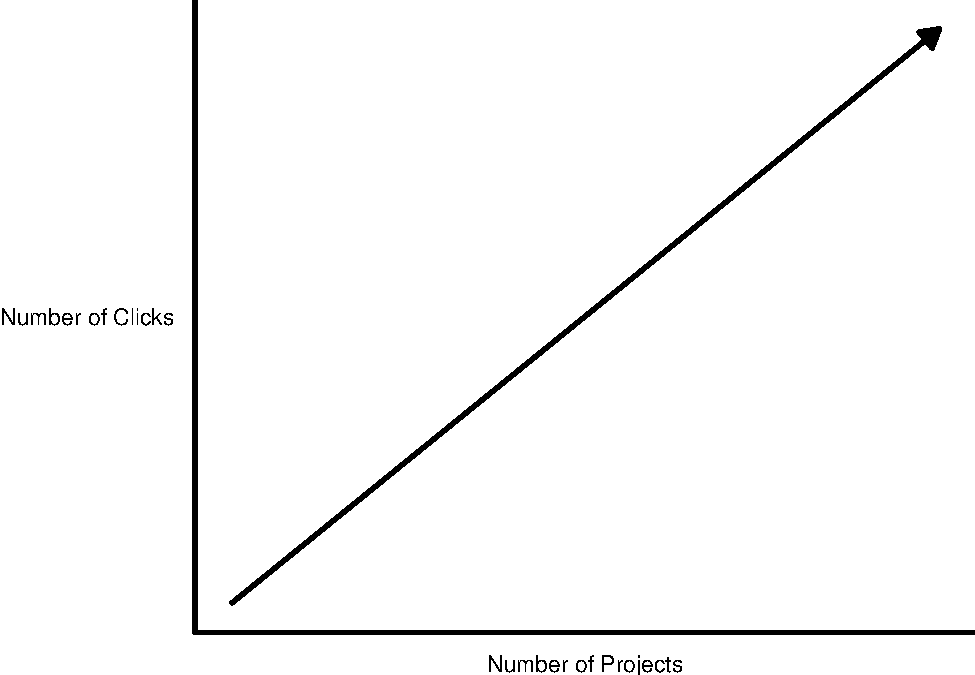
\includegraphics[width=1\linewidth]{introduction_files/figure-latex/unnamed-chunk-2-1}

Endless pointing and clicking was just one problem I faced using Excel. Annoying though it was, it didn't affect the quality of my work. Or so I thought until I recalled a project I had worked on a few years earlier.

In this project, I was looking at which school districts in the state of Oregon have \href{https://oregonstate.app.box.com/s/83g5sjdm88xgqdxfze0ri7qo4uff5sj7}{outdoor education programs known as Outdoor School}. As part of this project, I had to download data on all school districts throughout Oregon, filter to only include relevant districts with fifth or sixth graders (the ages Outdoor School takes place), and then merge this with data that I collected as part of a survey I conducted.

I did the work in Excel, using a lot of (you guessed it!) pointing and clicking. The problem came when I was almost done with the project. I've blocked the details from my memory (as I've done with most things Excel-related), but what I do recall is that not being 100\% certain I had done my filtering and joining correctly. And, to make it worse, I had no way to check my work. Why? Because all my pointing and clicking was ephemeral, gone in the ether as soon as I had completed it.

I finished the Outdoor School project and submitted my report. I think the work I did was \emph{probably} accurate, but maybe it wasn't?

Now, you may be reading this thinking: why didn't you write down the steps you used in Excel so you could retrace them later? Sure, I could (and should) have done that. But let's be honest: most of us don't.

The reality is, we're human. We all make mistakes. And without a straightforward way to audit your work (and keeping a list of all of your Excel points and clicks in a separate document is not, in my view, straightforward), mistakes will happen. If you've used Excel to work with data, I guarantee you've made a mistake, just like me.

The good news is that it's ok. There's a solution. And that solution is R.

If I were to redo that project on Outdoor School with R, here's what I'd do differently. Rather than watching points and clicks disappear into the ether, I'd write code that would serve as a record of everything I did. This code would:

Download data on all school districts:

Filter to only include districts with fifth or sixth graders:

Join the filtered data on school districts with my survey data:

Code can be scary. Having to write code is one of the reasons many people never learn R. But code is just a list of things you want to do to your data. It may be written in a hard-to-parse syntax (though it gets easier over time), but it's just a set of steps. The same steps that we should write out when we're working in Excel, but never do. Rather than having a separate document with my steps written down (the one that never gets written), I can see my steps in my code. See that line that says filter. Guess what it's doing? Yep, it's filtering!

If I had done things this way when working on the Outdoor School project, I could have looked back at any point to make sure what I thought was happening to my data was in fact happening. That nagging sensation I had near the end of the project that I may have made a mistake in one of my early points or clicks? It never would come up because I could just review my code to make sure it did what I thought it did. And if it didn't, I could rewrite and rerun my code to get updated results.

Using R won't mean you'll never make mistakes again (trust me, you will). But it will mean that you can easily spot your mistakes, make changes, and fix any issues.

I started learning R to avoid tedious pointing and clicking. But what I found was that R improved my work in ways I never expected. It's not just that my wrists are less tired. I now have more confidence that my work is accurate.

\begin{center}\rule{0.5\linewidth}{0.5pt}\end{center}

I used to feel ashamed about the way I use R.

I use R, a tool for statistical analysis, but I don't use it for complex statistical analysis. I don't do machine learning. I don't know what a random forest is. I've never even run a regression in R.

\href{https://rfortherestofus.com/2018/12/descriptive-stats-r/}{The only statistics I do in R are descriptive statistics}. Counts, sums, averages: these are the statistics that I do in R.

For a long time, I felt like I wasn't a ``real'' R user. Real R users, in my mind, used R for hardcore stats. I ``only'' used R for descriptive stats.

I sometimes felt like I was using a souped up sports car to drive 20 miles an hour to the grocery store. What was the point in using a high-powered machine like R to do ``simple'' things?

Eventually, I realized that this framing misses the point. \href{https://rss.onlinelibrary.wiley.com/doi/10.1111/j.1740-9713.2018.01169.x}{R started out as a tool created by statisticians for other statisticians}. But, over a quarter century since its creation, R can do much more than statistical analysis.

My own use of R is an example of this. I think of my work with R in three buckets:

\textbf{Illuminate} through data visualization: making graphs, maps, and tables that look good and share results effectively.

TODO: Add examples

\textbf{Communicate} by doing reporting with RMarkdown: moving away from the inefficiency and error-prone workflow of using multiple tools to create reports by instead doing it all in the one tool that I think of as \href{https://rfortherestofus.com/2019/03/r-killer-feature-rmarkdown/}{R's killer feature}.

TODO: Improve/explain graphics

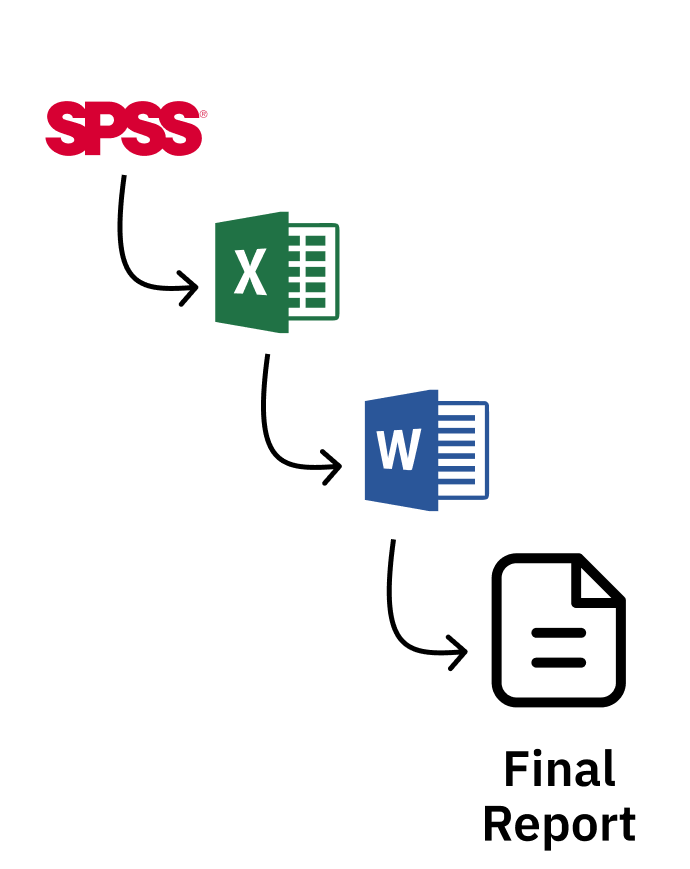
\includegraphics{assets/non-r-workflow.png}


\includegraphics{assets/r-workflow.png}

\textbf{Automate} tedious practices: Remember my Excel-burdened wrists? Since I moved to R I've found so many ways to automate tedious practices, from gathering data directly from the U.S. Census Bureau to pulling survey results in from Qualtrics and more.


\includegraphics{assets/qualtrics-workflow.png}

The main reason I've come to accept that my way of using R is as valid as anyone else's has come through realizing that more ``sophisticated'' R users are doing many of the same things I am. Sure, they may also be doing statistical analyses that I am not, but everyone who uses R needs to illuminate, communicate, and automate.

Canadian statistician Sharla Gelfand has \href{https://twitter.com/sharlagelfand/status/1135962094938009601}{talked about how they used R to automate an annual report on nursing registration exams in Ontario}. Sharla told me in 2019 that, despite being a statistician, \href{https://rfortherestofus.com/2019/09/my-r-journey-sharla-gelfand/}{the most statistical thing they did was calculating a median}.

Take a look at the R community on Twitter (where users congregate under the \#rstats hashtag). What gets people most excited is not the latest complex statistical analysis. \href{https://twitter.com/dgkeyes/status/1479473689225695234}{It's tips and tricks on the foundational work that everyone who uses R needs to do}. Things like:

\begin{itemize}
\item
  \href{https://twitter.com/CedScherer/status/1220843943224578050}{Making illuminating data visualizations} as part of the \href{https://github.com/rfordatascience/tidytuesday}{Tidy Tuesday project}.
\item
  \href{https://twitter.com/spcanelon/status/1424932510065209348}{Video tutorials on how to communicate through effective presentations using R}.
\item
  \href{https://twitter.com/WeAreRLadies/status/1228049014601342976}{Love letters to the \texttt{clean\_names()} function from the \texttt{janitor} package, which automates the process of making messy variable names easy to work with in R}.
\end{itemize}

No matter what else you do in R, you have to \textbf{illuminate} your findings and \textbf{communicate} your results. And, the more you use R, the more you'll find yourself wanting to \textbf{automate} things you used to do manually (your wrists will thank you).

I realize now that the things that I use R for \emph{are} the things that everyone uses R for. R was created for statistics. But today people are just as likely to use R without statistics.

Ten years ago, if you had told me I'd be writing a book on R, I'd have laughed. As someone with an extremely non-quantitative background (I did a PhD in anthropology) who never used R in graduate school, I never thought I'd be in a position to teach people about R. But here we find ourselves. And I'm excited to be your guide on this journey through the ways you can use R without statistics.

If I only used R for the things I thought ``real'' R users used it for, I wouldn't be writing this book. But, instead of slogging away in the world of complex statistical analysis, far outside of my area of expertise, I have found a place for myself in the world of R. Expanding my conception of what R can do has enabled me to get more out of this tool.

And here's the thing: if I, a qualitatively-trained anthropologist whose most complex statistical use for R is calculating averages, can find value in R, so can you. No matter what your background or what you think about R right now, using R without statistics can transform how you work in the future.

\hypertarget{how-this-book-works}{%
\section{How This Book Works}\label{how-this-book-works}}

This book shows the many ways that people use R without statistics. It's not comprehensive (trust me, there are many ways people use R not covered here). But I hope the ideas inspire you to think about learning to use R (if you're not yet an R user) or (if you are already on board the R train) learning to use R in ways you hadn't previously considered.

Each chapter focuses on one novel use of R. You'll begin by learning about a user or users who have transformed their work using R. You'll learn about a problem they had and how R helped them to solve it.We'll dive into their code, analyzing it line by line in order to help you understand how they used R. Each chapter will conclude with a short summary, offering lessons you can take from this novel way of using R.

I've tried to choose topics for each chapter that are relevant to a broad audience. Things like data visualization, report generation, and creating your own functions are things that anyone, no matter what you use R for, will find valuable.

There are some great topics that I thought to include but were just too narrow in their focus (for example, \href{https://blog.djnavarro.net/posts/2021-10-19_rtistry-posts/}{the world of generative art made with R}. If, at any point while you're reading this book, you think, ``why didn't David include X topic,'' please know that X might be a great topic, but I can only cover so much. The fact that you're able to come up with other ideas for things that R can do is a) fantastic and b) a further display of R's versatility. I eagerly await your follow-up book highlighting the myriad other things R can do that I am unable to cover in this book!

\hypertarget{a-favor-to-ask}{%
\section{A Favor to Ask}\label{a-favor-to-ask}}

Pedants of the world (as one of you, I come in peace), I have a favor to ask.

This book is called R Without Statistics. But it's not meant to be taken literally.

Of course it's true that if you're making a graph you're using statistics. So, before you start typing an angry email to me, please know that R Without Statistics is a mindset rather than a literal statement.

We're all using R with statistics already. Let's also learn to use R without statistics.

\hypertarget{part-illuminate}{%
\chapter{(PART*) Illuminate}\label{part-illuminate}}

\hypertarget{use-general-principles-of-high-quality-data-viz-in-r}{%
\chapter{Use General Principles of High-Quality Data Viz in R}\label{use-general-principles-of-high-quality-data-viz-in-r}}

In the spring of 2021, nearly all of the American West was in a drought. In April of that year, officials in Southern California declared a water emergency, citing unprecedented conditions.

This wouldn't have come as news to those living in California and other Western states. In addition to the direct impact of drought (leading areas of California to implement water use restrictions), people could see the indirect impact of drought in the skies. With forests dried out by years of drought conditions, wildfires became more frequent, filling the air with smoke. By the summer, there were be so many wildfires that smoke from drifted across the country, making even East Coast skies hazy and the air dangerous to breathe.

Drought conditions like those in the West in 2021 are becoming increasingly common. Yet communicating the extent of problem remains difficult. How can we show the data in a way that accurately represents the data while is also compelling enough to get people to take notice?

This was the challenge that data visualization designers Cédric Scherer and Georgios Karamanis took on in the fall of 2021. Commissioned by the magazine Scientific American to create a data visualization of drought conditions in the last two decades in the United States, they turned to the \texttt{ggplot2} package to turn what could be (pardon the pun) dry data into a visually arresting and impactful graph.

There was nothing unique about the data that Cédric and Georgios used. It was the same data from the National Drought Center that news organizations used in their stories. But Cédric and Georgios visualized the data in a way that it both grabs attention and communicates the scale of the phenomenon.

Below is a section of the final visualization (If you're incredibly eagle-eyed, you'll see a few minor elements that differ from the version published in Scientific American). These are things I had to change to make the plots fit in this book (e.g.~text size and putting legend text on two rows) or things that Scientific American added in post-production (e.g.~some annotations). Showing four regions over the last two decades, the increase in drought conditions, especially in California and the Southwest, is made apparent.

\begin{figure}
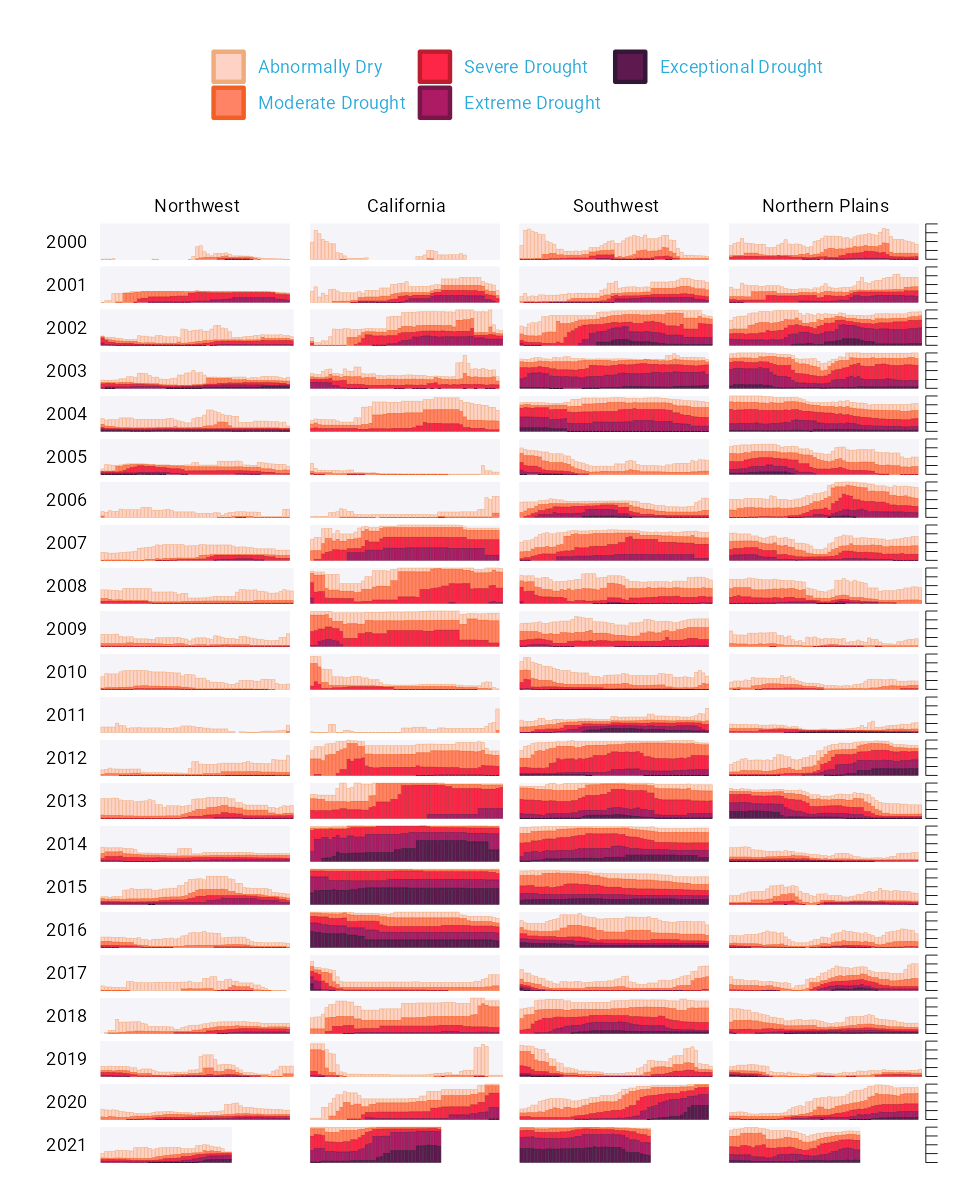
\includegraphics[width=1\linewidth]{data-viz_files/figure-latex/unnamed-chunk-3-1} \caption{Test}\label{fig:unnamed-chunk-3}
\end{figure}

To understand why this visualization is effective, let's break it down into pieces.

At the broadest level, the data viz is also notable for its minimalist aesthetic. There are, for example, no grid lines, little text along the axes, and few text labels. What Cédric and Georgios have done is to remove what statistician Edward Tufte, in his 1983 book \emph{The Visual Display of Quantitative Information}, calls ``chartjunk.'' Tufte wrote (and researchers as well as data viz designers since have generally agreed) that extraneous elements often hinder, rather than help, our understanding of charts.

Need proof that Cédric and Georgios's decluttered graph is better than the alternative? Here's a version with a few small tweaks to the code to include grid lines and text labels on axes. Prepare yourself for clutter!

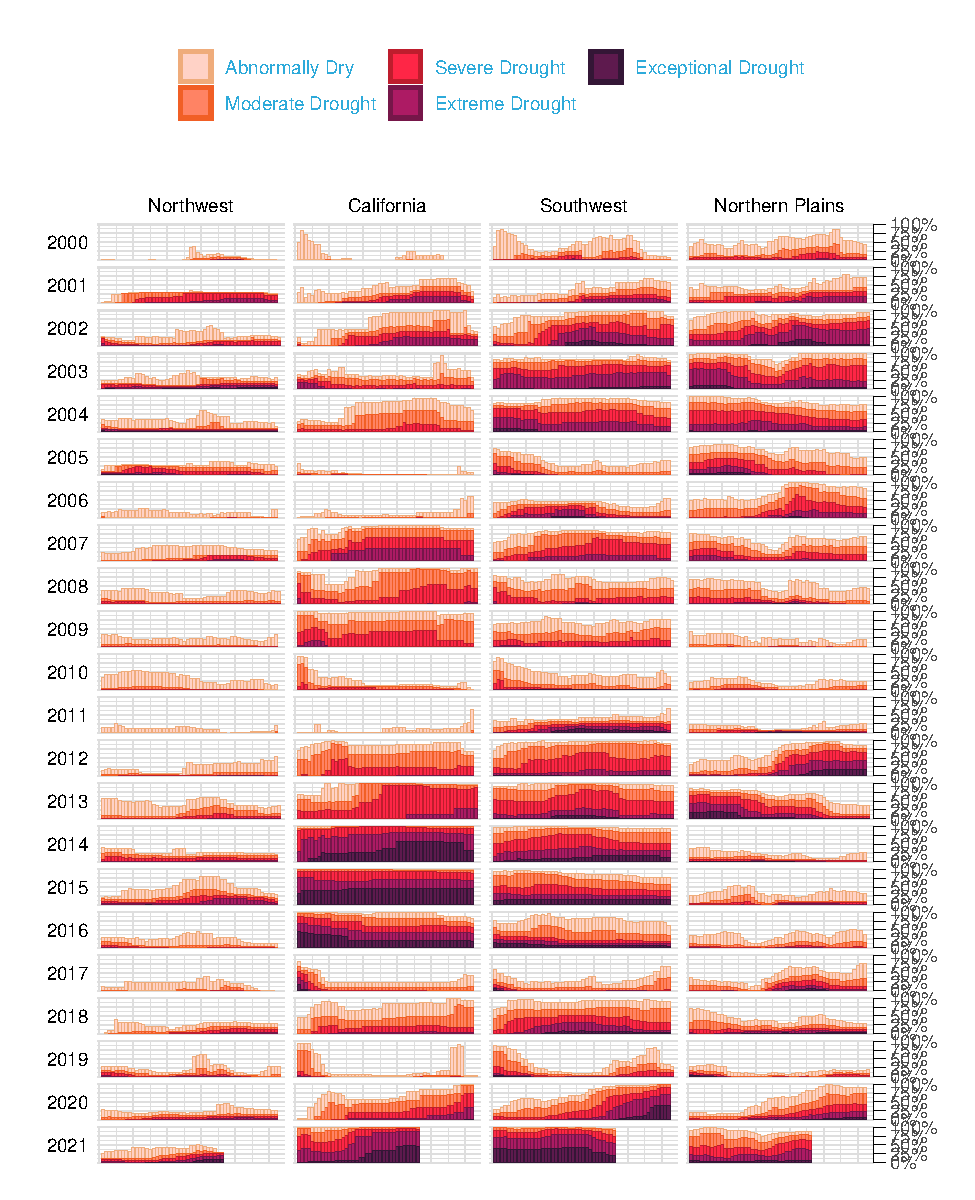
\includegraphics[width=1\linewidth]{data-viz_files/figure-latex/unnamed-chunk-4-1}

And, again, it's not just that this cluttered version looks worse. The clutter actively inhibits understanding. Rather than focus on overall drought patterns (the point of the graph), our brain gets stuck reading repetitive and unnecessary axis text.

One of the best ways to reduce clutter is to break a single chart into what are known as small multiples. When we look closely at the data viz, we see that it is not one chart but actually a set of charts. Each rectangle represents one region in one year. If we filter to show the Southwest region in 2003 and add axis titles, we can see that the x axis shows the week while the y axis shows the percentage of that region at different drought levels.

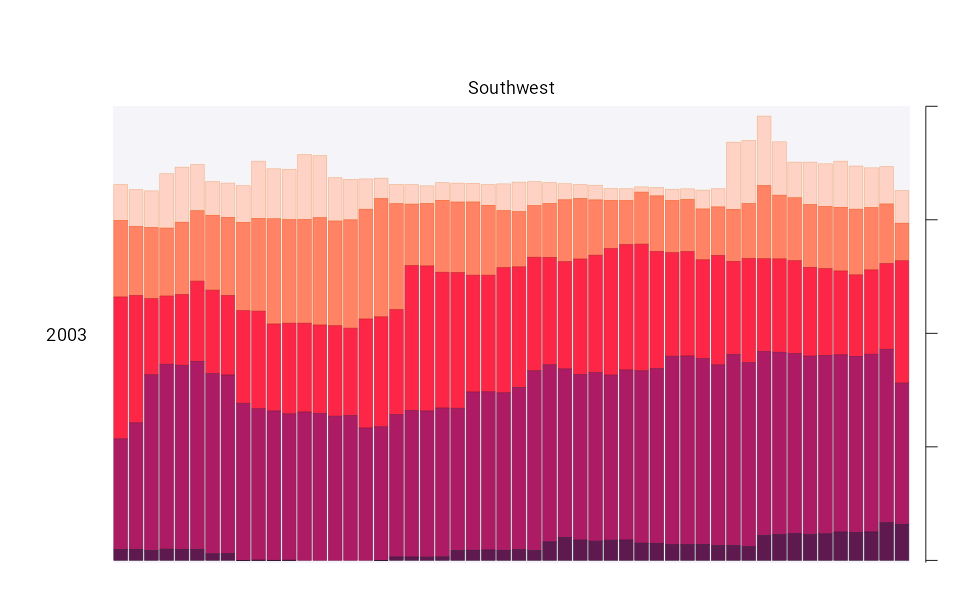
\includegraphics[width=1\linewidth]{data-viz_files/figure-latex/unnamed-chunk-5-1}

Zooming in on a single region in a single year also makes the color choices more obvious. The lightest bars show the percentage of the region that is abnormally dry while the darkest bars shows the percentage in exceptional drought conditions. These colors, as we'll see shortly, are intentionally chosen to make differences in the drought levels visible to all readers.

When I asked Cédric and Georgios to speak with me about this data visualization, they initially told me that the code for this piece might be too simple to highlight the power of R for data viz.~No, I told them, I want to speak with you precisely \emph{because} the code is not super complex. The fact that Cédric and Georgios were able to produce this complex graph with relatively simple code shows the power of R for data visualization. And it is possible because of a theory called the grammar of graphics.

\hypertarget{the-grammar-of-graphics}{%
\section{The Grammar of Graphics}\label{the-grammar-of-graphics}}

If you've used Excel to make graphs, you're probably familiar with this menu:

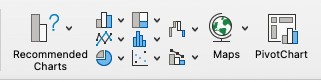
\includegraphics[width=1\linewidth]{assets/excel-chart-chooser}

Working in Excel, your graph-making journey begins with the step of selecting the type of graph you want to make. Want a bar chart? Click the bar chart icon. Want a line chart? Click the line chart icon.

If you've only ever made data visualization in Excel, this first step may seem so obvious that you've never even considered conceptualizing the process of creating data visualization in any different way. This was certainly the case for me in my years as an Excel user.

But there are different ways to think about graphs. Rather than conceptualizing graphs types as being distinct, it is also possible to recognize the things that they have in common, and using these commonalities as the starting point for making graphs.

This approach to thinking about graphs comes from the late statistician Leland Wilkinson. Wilkinson thought deeply for years about what data visualization is and how we can describe it. In 1999, he published a book called \emph{The Grammar of Graphics} that sought to develop a consistent way of describing \emph{all} graphs.

Wilkinson argued that we should think of plots not as distinct types a la Excel, but as following a grammar that we can use to describe \emph{any} plot. Throughout the book that Wilkinson is best remembered for, he presented general principles to describe graphs. Just as knowledge of English grammar tells us that a noun is typically followed by a verb (``he goes'') works while the opposite (``goes he'') does not, knowledge of the grammar of graphics allows us to understand why certain graph types ``work.'' Or, as Wilkinson put it,

\begin{quote}
A language consisting of words and no grammar (statement = word) expresses only as many ideas as there are words. \ldots{} The grammar of graphics takes us beyond a limited set of charts (words) to an almost unlimited world of graphical forms (statements).
\end{quote}

Thinking about data visualization through the lens of the grammar of graphics allow us to see, for example, that graphs typically have data that is plotted on the x axis and other data that is plotted on the y axis. And this is the case no matter whether the type of graph we end up with is, to take just two examples, a bar chart of a line chart. Consider these two graphs, which use data on life expectancy in Afghanistan:

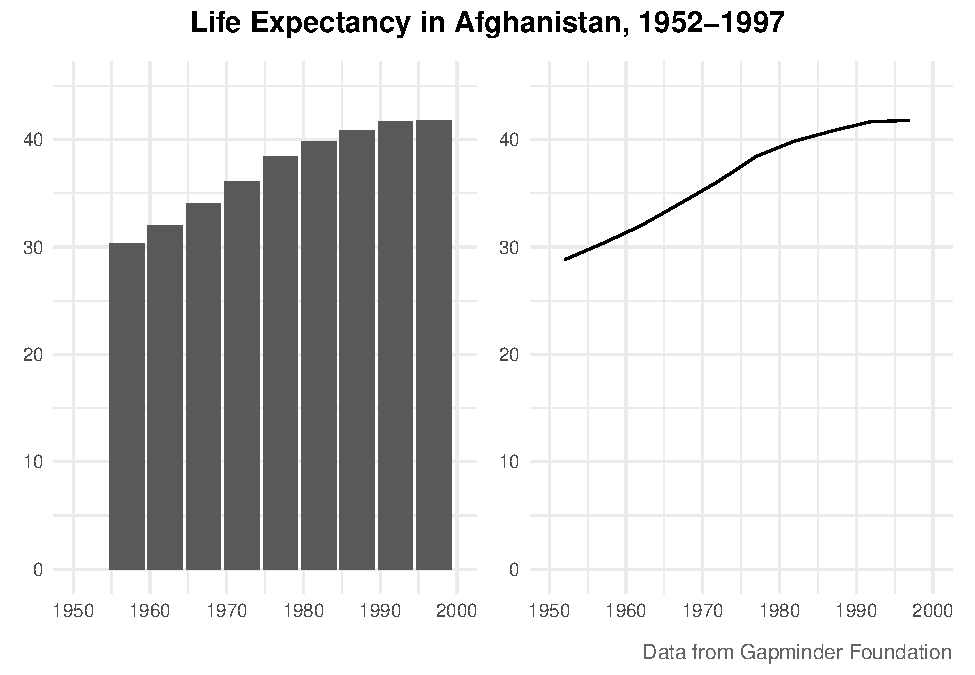
\includegraphics[width=1\linewidth]{data-viz_files/figure-latex/unnamed-chunk-7-1}

While they look different (and would, to the Excel user, be different types of graphs), Wilkinson's grammar of graphics allows us to see their similarities.

As an academic statistician, Wilkinson's goal in writing \emph{The Grammar of Graphics} was to provide a novel way of thinking about data visualization. But his feelings on graph-making tools like Excel were clear when he wrote that ``most charting packages channel user requests into a rigid array of chart types.''

At the time Wilkinson wrote his book, there was no data viz tool that could implement his grammar of graphics. This would change in 2010, when Hadley Wickham announced the \texttt{ggplot2} package for R. Providing the tools to implement Wilkinson's ideas, \texttt{ggplot2} would come to revolutionize the world of data visualization.

\hypertarget{ggplot2}{%
\section{ggplot2}\label{ggplot2}}

Hadley Wickham's article announcing \texttt{ggplot2} (which I, like nearly everyone in the data viz world, will refer to simply as ggplot) was titled \emph{A Layered Grammar of Graphics}. It showed a new R package that relied on the grammar of graphics and added on the idea of plots having multiple layers. Let's walk through some of the most important layers.

When creating a graph with ggplot, we begin by mapping data to aesthetic properties. To the uninitiated, this may sound like complete nonsense. But all it means is that we use things like the x or y axis, color, size (aka aesthetic properties) to represent variables.

Let's make this concrete using the same data on life expectancy in Afghanistan. Here's what this data looks like.

\begin{verbatim}
#> # A tibble: 10 x 6
#>    country     continent  year lifeExp      pop gdpPercap
#>    <fct>       <fct>     <int>   <dbl>    <int>     <dbl>
#>  1 Afghanistan Asia       1952    28.8  8425333      779.
#>  2 Afghanistan Asia       1957    30.3  9240934      821.
#>  3 Afghanistan Asia       1962    32.0 10267083      853.
#>  4 Afghanistan Asia       1967    34.0 11537966      836.
#>  5 Afghanistan Asia       1972    36.1 13079460      740.
#>  6 Afghanistan Asia       1977    38.4 14880372      786.
#>  7 Afghanistan Asia       1982    39.9 12881816      978.
#>  8 Afghanistan Asia       1987    40.8 13867957      852.
#>  9 Afghanistan Asia       1992    41.7 16317921      649.
#> 10 Afghanistan Asia       1997    41.8 22227415      635.
\end{verbatim}

If we want to make a chart with ggplot, we need to first decide which variable to use to put on the x axis and which to put on the y axis. Let's say we want to show life expectancy over time. That means using the variable \texttt{year} on the x axis and the variable \texttt{lifeExp} on the y axis.

I begin by using the \texttt{ggplot()} function. Within this, I tell R that I'm using the data frame \texttt{gapminder\_10\_rows} (this is the filtered version I created from the full \texttt{gapminder} data frame, which includes over 1,700 rows of data). The line following this tells R to use \texttt{year} on the x and \texttt{lifeExp} on the y axis.

\begin{Shaded}
\begin{Highlighting}[]
\FunctionTok{ggplot}\NormalTok{(}
  \AttributeTok{data =}\NormalTok{ gapminder\_10\_rows,}
  \AttributeTok{mapping =} \FunctionTok{aes}\NormalTok{(}
    \AttributeTok{x =}\NormalTok{ year,}
    \AttributeTok{y =}\NormalTok{ lifeExp}
\NormalTok{  )}
\NormalTok{)}
\end{Highlighting}
\end{Shaded}

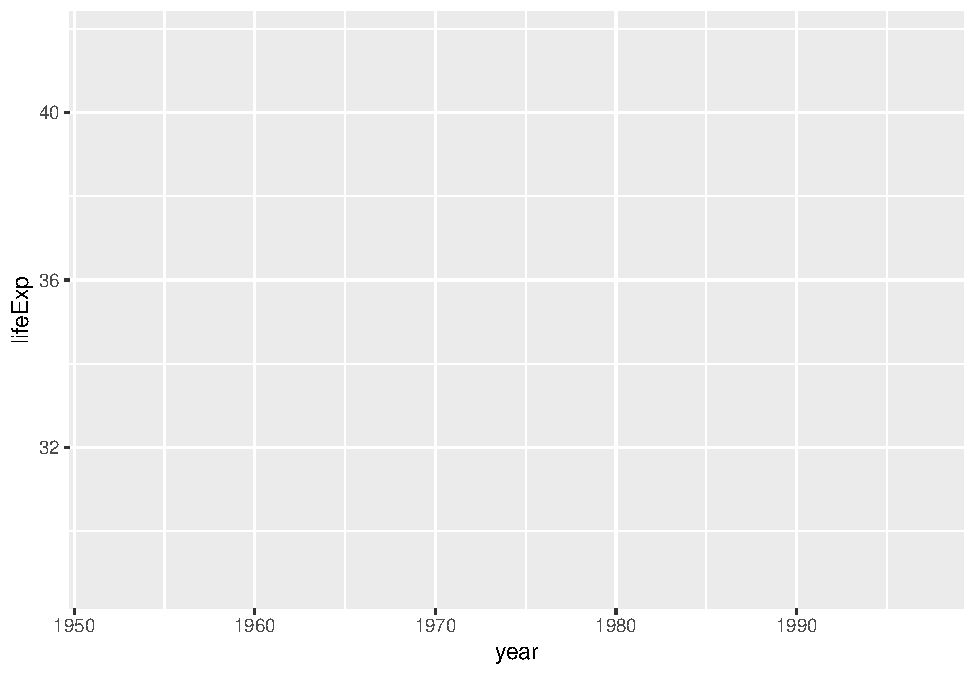
\includegraphics[width=1\linewidth]{data-viz_files/figure-latex/unnamed-chunk-9-1}

When I run my code, what I get doesn't look like much.

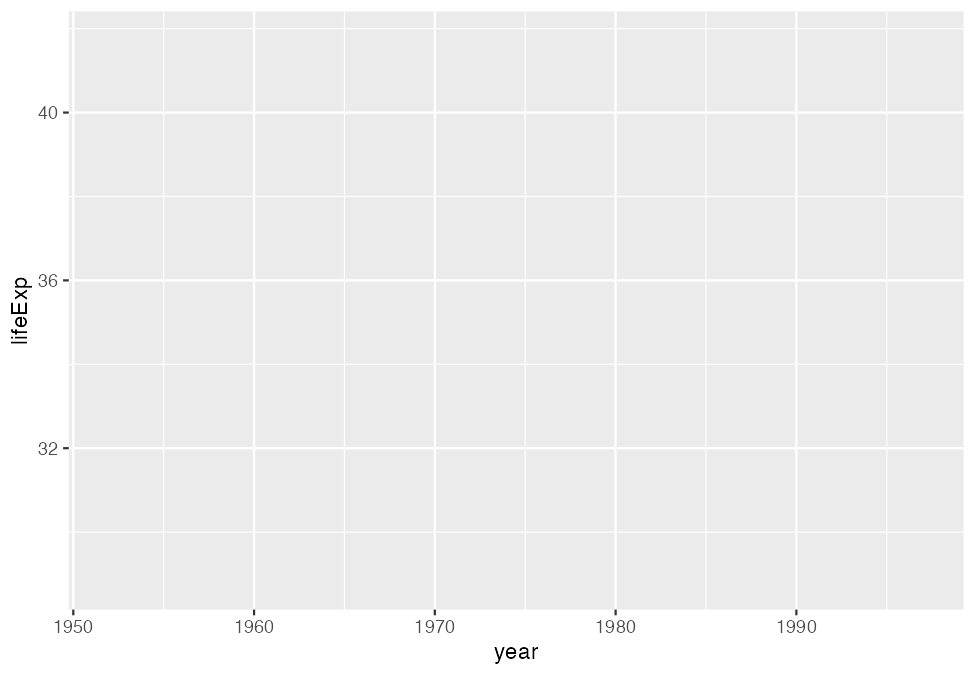
\includegraphics[width=1\linewidth]{data-viz_files/figure-latex/unnamed-chunk-11-1}

But if I look closely, I can see the beginnings of a plot. Remember that x axis using \texttt{year}? There it is! And \texttt{lifeExp} on the y axis? Yup, it's there too.

I can also see that the values on the x and y axes match up to our data. In the \texttt{gapminder\_10\_rows} data frame, the first year is 1952 and the last year is 1997. The range of the x axis seems to have been created with this data in mind (spoiler: it was). And \texttt{lifeExp}, which goes from about 28 to about 42 will fit nicely on our y axis.

Axes are nice, but we're missing any type of visual representation of the data. To get this, we need to add the next layer in ggplot: geoms. Short for geometric objects, geoms are different ways of representing data. For example, if we want to add points, we use \texttt{geom\_point()}.

\begin{Shaded}
\begin{Highlighting}[]
\FunctionTok{ggplot}\NormalTok{(}
  \AttributeTok{data =}\NormalTok{ gapminder\_10\_rows,}
  \AttributeTok{mapping =} \FunctionTok{aes}\NormalTok{(}
    \AttributeTok{x =}\NormalTok{ year,}
    \AttributeTok{y =}\NormalTok{ lifeExp}
\NormalTok{  )}
\NormalTok{) }\SpecialCharTok{+}
  \FunctionTok{geom\_point}\NormalTok{()}
\end{Highlighting}
\end{Shaded}

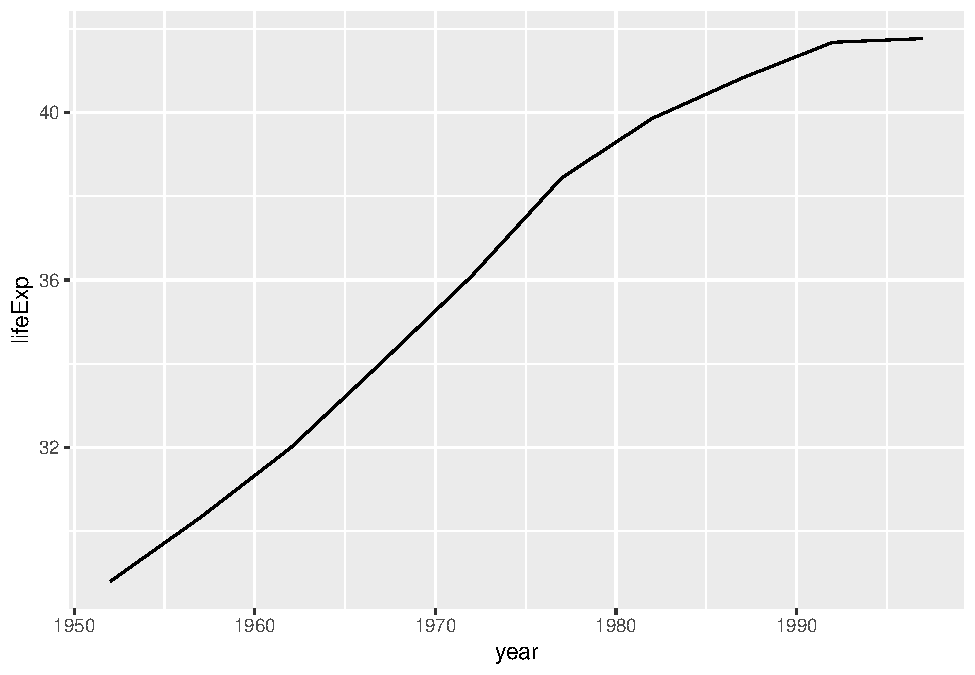
\includegraphics[width=1\linewidth]{data-viz_files/figure-latex/unnamed-chunk-12-1}

There we go! 1952 shows the life expectancy of about 28 and so on through every year in our data.

Let's say we change our mind and want to make a line chart instead. Well, all we have to do is replace \texttt{geom\_point()} with \texttt{geom\_line()}.

\begin{Shaded}
\begin{Highlighting}[]
\FunctionTok{ggplot}\NormalTok{(}
  \AttributeTok{data =}\NormalTok{ gapminder\_10\_rows,}
  \AttributeTok{mapping =} \FunctionTok{aes}\NormalTok{(}
    \AttributeTok{x =}\NormalTok{ year,}
    \AttributeTok{y =}\NormalTok{ lifeExp}
\NormalTok{  )}
\NormalTok{) }\SpecialCharTok{+}
  \FunctionTok{geom\_line}\NormalTok{()}
\end{Highlighting}
\end{Shaded}

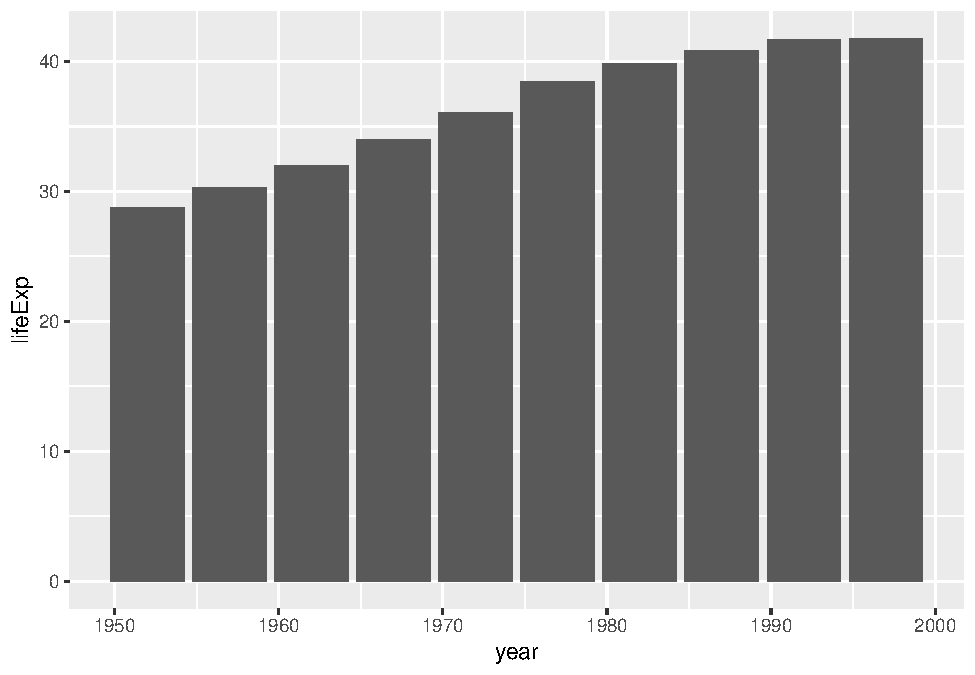
\includegraphics[width=1\linewidth]{data-viz_files/figure-latex/unnamed-chunk-14-1}

Or (and now we're really getting fancy), what if we add \emph{both} \texttt{geom\_point()} and \texttt{geom\_line()}? A line chart with points!

\begin{Shaded}
\begin{Highlighting}[]
\FunctionTok{ggplot}\NormalTok{(}
  \AttributeTok{data =}\NormalTok{ gapminder\_10\_rows,}
  \AttributeTok{mapping =} \FunctionTok{aes}\NormalTok{(}
    \AttributeTok{x =}\NormalTok{ year,}
    \AttributeTok{y =}\NormalTok{ lifeExp}
\NormalTok{  )}
\NormalTok{) }\SpecialCharTok{+}
  \FunctionTok{geom\_point}\NormalTok{() }\SpecialCharTok{+}
  \FunctionTok{geom\_line}\NormalTok{()}
\end{Highlighting}
\end{Shaded}

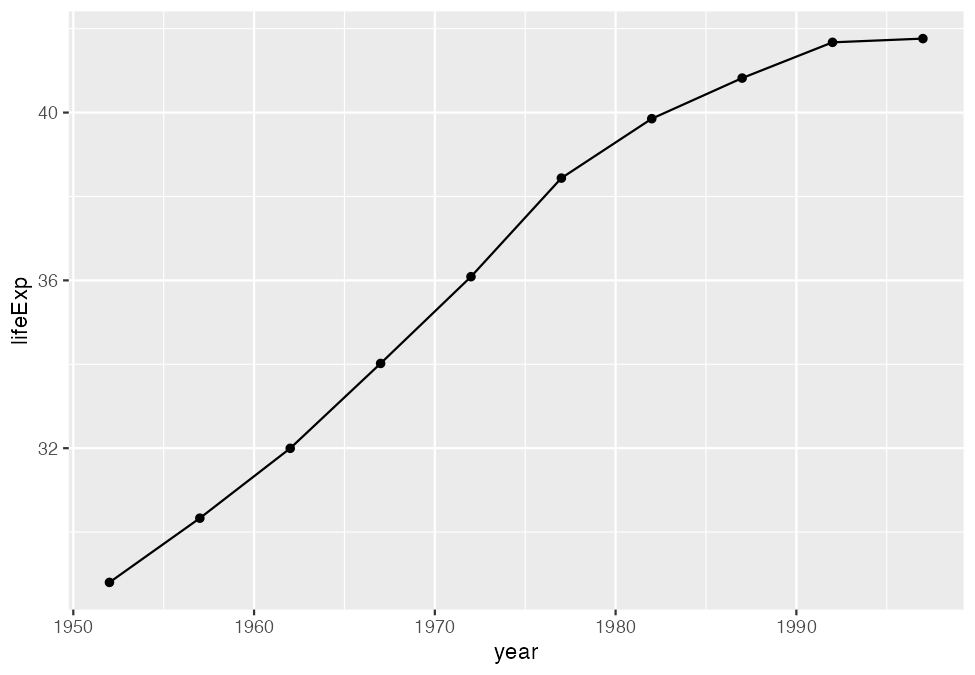
\includegraphics[width=1\linewidth]{data-viz_files/figure-latex/unnamed-chunk-16-1}

We can extend this idea further, swapping in \texttt{geom\_col()} to create to a bar chart (note that the y axis range has been automatically updated now, going from 0 to 40 to account for the different geom).

\begin{Shaded}
\begin{Highlighting}[]
\FunctionTok{ggplot}\NormalTok{(}
  \AttributeTok{data =}\NormalTok{ gapminder\_10\_rows,}
  \AttributeTok{mapping =} \FunctionTok{aes}\NormalTok{(}
    \AttributeTok{x =}\NormalTok{ year,}
    \AttributeTok{y =}\NormalTok{ lifeExp}
\NormalTok{  )}
\NormalTok{) }\SpecialCharTok{+}
  \FunctionTok{geom\_col}\NormalTok{()}
\end{Highlighting}
\end{Shaded}

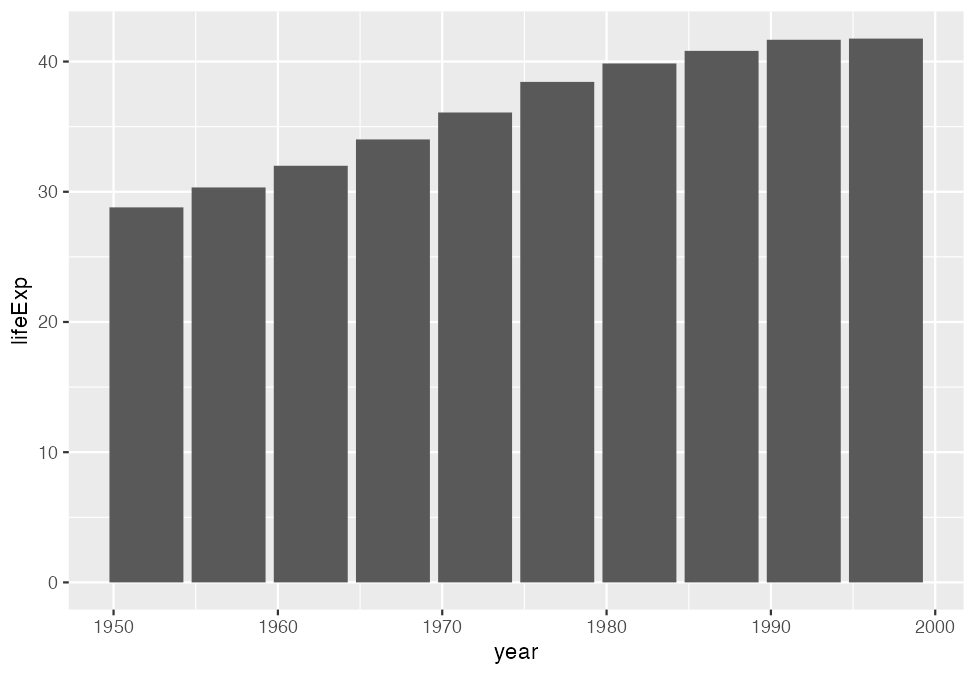
\includegraphics[width=1\linewidth]{data-viz_files/figure-latex/unnamed-chunk-18-1}

I hope you're seeing how ggplot is a direct implementation of Wilkinson's grammar of graphics. The difference between a line chart and a bar chart isn't as great as the Excel chart type picker might have us think. Both can have the same aesthetic properties (namely, putting year on the x axis and life expectancy on the y axis), but simply use different geometric objects to visually represent the data.

Before we return to the drought data viz, let's look at a few additional layers that can help us can alter our bar chart. Let's say we want to change the color of our bars. In the grammar of graphics approach to chart-making, this means mapping some variable to the aesthetic property of fill (slightly confusingly, the aesthetic property ``color'' would, for a bar chart, change the outline of each bar). In the same way that we mapped \texttt{year} to the x axis and y to \texttt{lifeExp}, we can also map fill to a variable. Let's try mapping fill to the year variable.

\begin{Shaded}
\begin{Highlighting}[]
\FunctionTok{ggplot}\NormalTok{(}
  \AttributeTok{data =}\NormalTok{ gapminder\_10\_rows,}
  \AttributeTok{mapping =} \FunctionTok{aes}\NormalTok{(}
    \AttributeTok{x =}\NormalTok{ year,}
    \AttributeTok{y =}\NormalTok{ lifeExp,}
    \AttributeTok{fill =}\NormalTok{ year}
\NormalTok{  )}
\NormalTok{) }\SpecialCharTok{+}
  \FunctionTok{geom\_col}\NormalTok{()}
\end{Highlighting}
\end{Shaded}

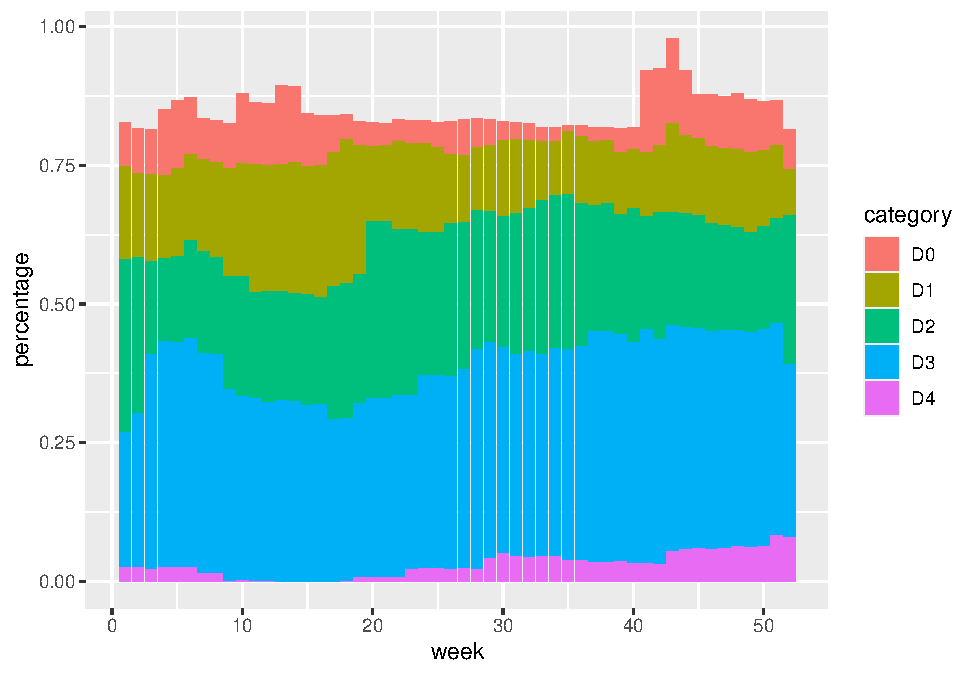
\includegraphics[width=1\linewidth]{data-viz_files/figure-latex/unnamed-chunk-20-1}

What we see now is that, for earlier years, the fill is darker while for later years, it is lighter (the legend, added to the right of our plot, shows this). What if we want to change the fill colors? For that, we use a new scale layer. In this case, I'll use the \texttt{scale\_fill\_viridis\_c()} function (the c at the end of the function name refers to the fact that the data is continuous). This function, just one of many functions that start with \texttt{scale\_} and can alter the fill scale, changes the default palette to one that is colorblind-friendly and prints well in grayscale.

\begin{Shaded}
\begin{Highlighting}[]
\FunctionTok{ggplot}\NormalTok{(}
  \AttributeTok{data =}\NormalTok{ gapminder\_10\_rows,}
  \AttributeTok{mapping =} \FunctionTok{aes}\NormalTok{(}
    \AttributeTok{x =}\NormalTok{ year,}
    \AttributeTok{y =}\NormalTok{ lifeExp,}
    \AttributeTok{fill =}\NormalTok{ year}
\NormalTok{  )}
\NormalTok{) }\SpecialCharTok{+}
  \FunctionTok{geom\_col}\NormalTok{() }\SpecialCharTok{+}
  \FunctionTok{scale\_fill\_viridis\_c}\NormalTok{()}
\end{Highlighting}
\end{Shaded}

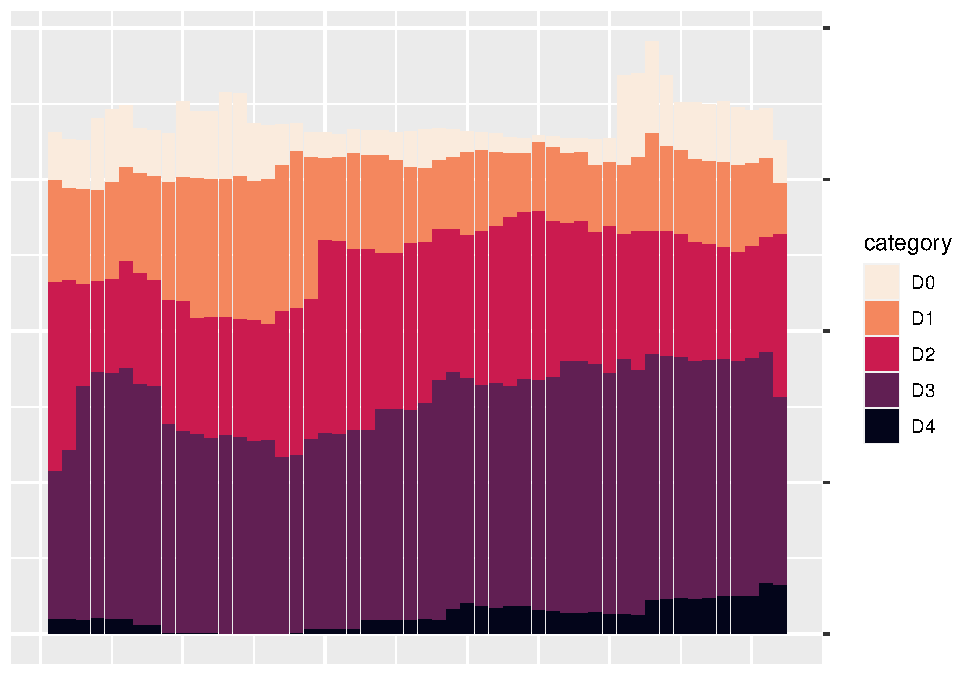
\includegraphics[width=1\linewidth]{data-viz_files/figure-latex/unnamed-chunk-22-1}

A final layer we'll look at is the theme layer. This layer allows us to change the overall look-and-feel of plots (think: plot backgrounds, grid lines, etc). Just as there are a number of \texttt{scale\_} functions, there are also a number of functions that start with \texttt{theme\_}. Below, I've added \texttt{theme\_minimal()}, which starts to declutter our plot.

\begin{Shaded}
\begin{Highlighting}[]
\FunctionTok{ggplot}\NormalTok{(}
  \AttributeTok{data =}\NormalTok{ gapminder\_10\_rows,}
  \AttributeTok{mapping =} \FunctionTok{aes}\NormalTok{(}
    \AttributeTok{x =}\NormalTok{ year,}
    \AttributeTok{y =}\NormalTok{ lifeExp,}
    \AttributeTok{fill =}\NormalTok{ year}
\NormalTok{  )}
\NormalTok{) }\SpecialCharTok{+}
  \FunctionTok{geom\_col}\NormalTok{() }\SpecialCharTok{+}
  \FunctionTok{scale\_fill\_viridis\_c}\NormalTok{() }\SpecialCharTok{+}
  \FunctionTok{theme\_minimal}\NormalTok{()}
\end{Highlighting}
\end{Shaded}

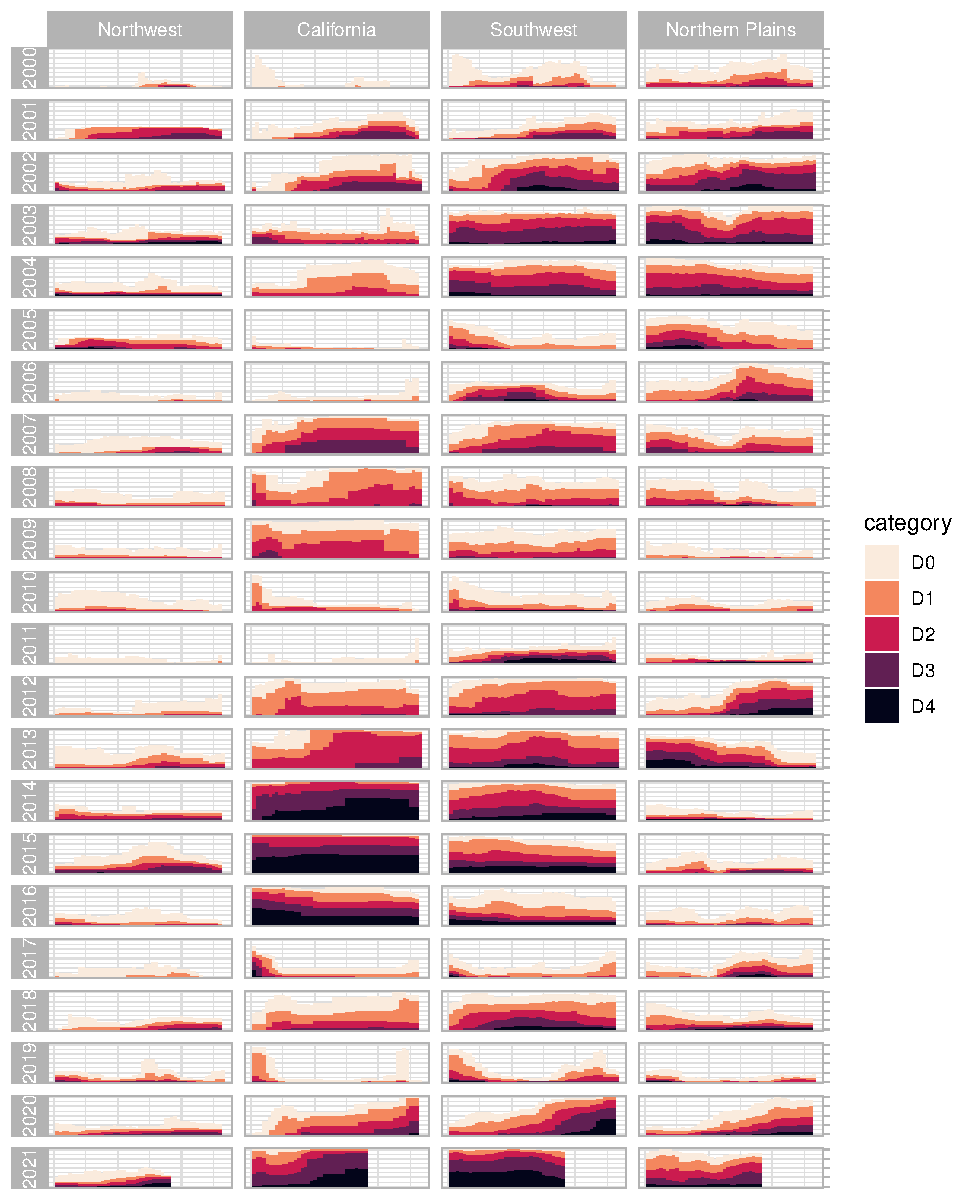
\includegraphics[width=1\linewidth]{data-viz_files/figure-latex/unnamed-chunk-24-1}

We've now seen why Hadley Wickham described the \texttt{ggplot2} package as using a layered grammar of graphics. It relies on Leland Wilkinson's theory and implements it through the creation of multiple layers:

\begin{itemize}
\tightlist
\item
  First, we select variables to map to aesthetic properties such as x or y axis, color/fill, etc
\item
  Second, we choose the geometric object (aka geom) we want to use to represent our data
\item
  Third, if we want to change aesthetic properties (for example, using a different palette), we do this with a \texttt{scale\_} function
\item
  Fourth, we use a \texttt{theme\_} function to set the overall look-and-feel of our plot.
\end{itemize}

There are many ways we could improve the plot we've been working on. But rather than improving an ugly plot, let's instead return to the drought data viz that Cédric Scherer and Georgios Karamanis made. Going through their code will show us some familiar aspects of ggplot -- and present some tips on how to make high-quality data visualization with R.

\hypertarget{recreating-the-drought-visualization}{%
\section{Recreating the Drought Visualization}\label{recreating-the-drought-visualization}}

The code that Cédric and Georgios wrote to make their final data viz relies on a combination of ggplot fundamentals and some less-well-known tweaks that make it really shine. In order to understand how Cédric and Georgios made their data viz, we'll start out with a simplified version of their code. We'll build it up layer by layer, adding elements until we can see exactly how they made their drought data viz.~

Let's start by looking again at one region (Southwest) in one year (2003). First, we filter our data and save it as a new object called \texttt{southwest\_2003}.

\begin{Shaded}
\begin{Highlighting}[]
\NormalTok{southwest\_2003 }\OtherTok{\textless{}{-}}\NormalTok{ dm\_perc\_cat\_hubs }\SpecialCharTok{\%\textgreater{}\%}
  \FunctionTok{filter}\NormalTok{(hub }\SpecialCharTok{==} \StringTok{"Southwest"}\NormalTok{) }\SpecialCharTok{\%\textgreater{}\%}
  \FunctionTok{filter}\NormalTok{(year }\SpecialCharTok{==} \DecValTok{2003}\NormalTok{)}
\end{Highlighting}
\end{Shaded}

We can take a look at this object to see the variables we have to work with:

\begin{itemize}
\tightlist
\item
  \textbf{date}: start date of the week of the observation
\item
  \textbf{hub}: region
\item
  \textbf{category}: level of drought (D0 = lowest level of drought; D5 = highest level)
\item
  \textbf{percentage}: percentage of that region that is in that category of drought (0 = 0\%, 1 = 100\%)
\item
  \textbf{year}: observation year
\item
  \textbf{week}: week number (i.e.~first week is week 1)
\item
  \textbf{max\_week}: the maximum number of weeks in a given year
\end{itemize}

\begin{Shaded}
\begin{Highlighting}[]
\NormalTok{southwest\_2003 }\SpecialCharTok{\%\textgreater{}\%}
  \FunctionTok{slice}\NormalTok{(}\DecValTok{1}\SpecialCharTok{:}\DecValTok{10}\NormalTok{)}
\CommentTok{\#\textgreater{} \# A tibble: 10 x 7}
\CommentTok{\#\textgreater{}    date       hub       category perce\textasciitilde{}1  year  week max\_w\textasciitilde{}2}
\CommentTok{\#\textgreater{}    \textless{}date\textgreater{}     \textless{}fct\textgreater{}     \textless{}fct\textgreater{}      \textless{}dbl\textgreater{} \textless{}dbl\textgreater{} \textless{}dbl\textgreater{}   \textless{}dbl\textgreater{}}
\CommentTok{\#\textgreater{}  1 2003{-}12{-}30 Southwest D0        0.0718  2003    52      52}
\CommentTok{\#\textgreater{}  2 2003{-}12{-}30 Southwest D1        0.0828  2003    52      52}
\CommentTok{\#\textgreater{}  3 2003{-}12{-}30 Southwest D2        0.269   2003    52      52}
\CommentTok{\#\textgreater{}  4 2003{-}12{-}30 Southwest D3        0.311   2003    52      52}
\CommentTok{\#\textgreater{}  5 2003{-}12{-}30 Southwest D4        0.0796  2003    52      52}
\CommentTok{\#\textgreater{}  6 2003{-}12{-}23 Southwest D0        0.0823  2003    51      52}
\CommentTok{\#\textgreater{}  7 2003{-}12{-}23 Southwest D1        0.131   2003    51      52}
\CommentTok{\#\textgreater{}  8 2003{-}12{-}23 Southwest D2        0.189   2003    51      52}
\CommentTok{\#\textgreater{}  9 2003{-}12{-}23 Southwest D3        0.382   2003    51      52}
\CommentTok{\#\textgreater{} 10 2003{-}12{-}23 Southwest D4        0.0828  2003    51      52}
\CommentTok{\#\textgreater{} \# ... with abbreviated variable names 1: percentage,}
\CommentTok{\#\textgreater{} \#   2: max\_week}
\end{Highlighting}
\end{Shaded}

Now we can use this \texttt{southwest\_2003} object for our plotting. In the \texttt{ggplot()} function, we tell R to put week on the x axis, percentage on the y axis, and use the category variable (i.e.~drought level) for our fill color. We then use \texttt{geom\_col()} to create a bar chart where the fill color of each bar represents the percentage of the region in a single week that is at different drought levels. The colors don't match the final version of the plot, but with this code we can start to see the outlines of Cédric and Georgios's data viz.~

\begin{Shaded}
\begin{Highlighting}[]
\FunctionTok{ggplot}\NormalTok{(}
  \AttributeTok{data =}\NormalTok{ southwest\_2003,}
  \FunctionTok{aes}\NormalTok{(}
    \AttributeTok{x =}\NormalTok{ week,}
    \AttributeTok{y =}\NormalTok{ percentage,}
    \AttributeTok{fill =}\NormalTok{ category}
\NormalTok{  )}
\NormalTok{) }\SpecialCharTok{+}
  \FunctionTok{geom\_col}\NormalTok{()}
\end{Highlighting}
\end{Shaded}

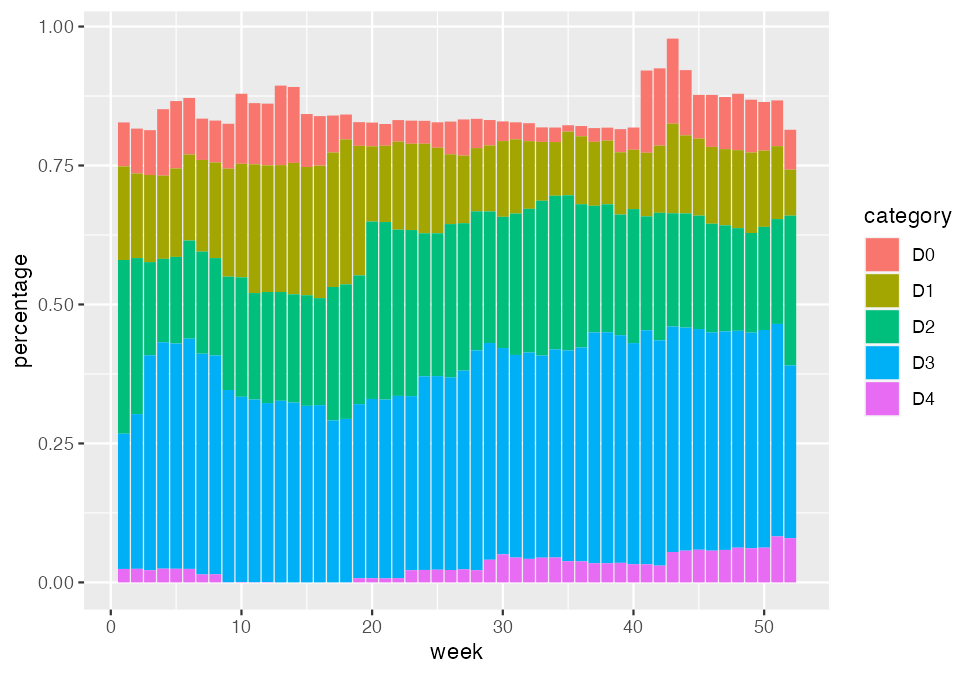
\includegraphics[width=1\linewidth]{data-viz_files/figure-latex/unnamed-chunk-28-1}

Cédric and Georgios next select different fill colors for their bars. They use the \texttt{scale\_fill\_viridis\_d()} function. The ``d'' here means the data that the fill scale is being applied to has discrete categories (D0, D1, D2, D3, D4, D5). They use the argument \texttt{option\ =\ "rocket"} in order to select the ``rocket'' palette (the \texttt{scale\_fill\_viridis\_d()} function has several other palettes). And they use the \texttt{direction\ =\ -1} argument to reverse the order of fill colors so that darker colors mean higher drought conditions.

\begin{Shaded}
\begin{Highlighting}[]
\FunctionTok{ggplot}\NormalTok{(}
  \AttributeTok{data =}\NormalTok{ southwest\_2003,}
  \FunctionTok{aes}\NormalTok{(}
    \AttributeTok{x =}\NormalTok{ week,}
    \AttributeTok{y =}\NormalTok{ percentage,}
    \AttributeTok{fill =}\NormalTok{ category}
\NormalTok{  )}
\NormalTok{) }\SpecialCharTok{+}
  \FunctionTok{geom\_col}\NormalTok{() }\SpecialCharTok{+}
  \FunctionTok{scale\_fill\_viridis\_d}\NormalTok{(}
    \AttributeTok{option =} \StringTok{"rocket"}\NormalTok{,}
    \AttributeTok{direction =} \SpecialCharTok{{-}}\DecValTok{1}
\NormalTok{  )}
\end{Highlighting}
\end{Shaded}

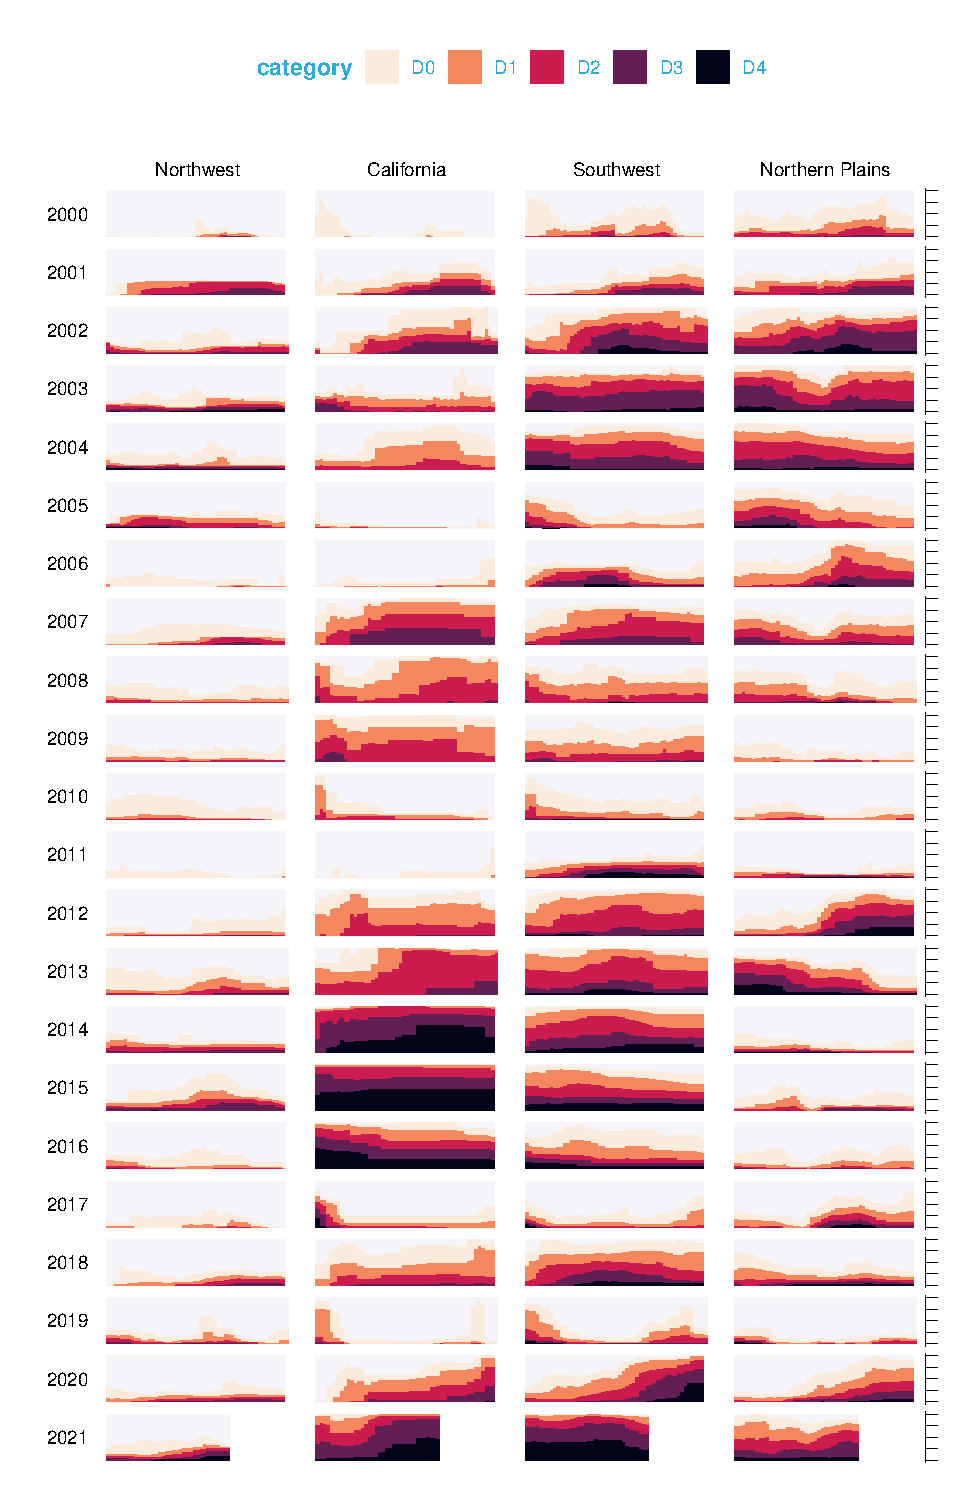
\includegraphics[width=1\linewidth]{data-viz_files/figure-latex/unnamed-chunk-30-1}

In the language of ggplot, x and y axis are aesthetic properties, the same as fill color. Cédric and Georgios tweak the x axis to remove both the axis title (``week'') using \texttt{name\ =\ NULL} and the 0-50 axis text with \texttt{guide\ =\ none}. On the y axis, they remove the axis title and axis text (which was showing percentages in 0.00, 0.25, 0.50, 0.75 format) using \texttt{labels\ =\ NULL} (this functionally does the same thing as \texttt{guide\ =\ "none"}). They also move the axis lines themselves to the right side using \texttt{position\ =\ "right"} (they are only apparent as tick marks at this point, but will become more visible later).

\begin{Shaded}
\begin{Highlighting}[]
\FunctionTok{ggplot}\NormalTok{(}
  \AttributeTok{data =}\NormalTok{ southwest\_2003,}
  \FunctionTok{aes}\NormalTok{(}
    \AttributeTok{x =}\NormalTok{ week,}
    \AttributeTok{y =}\NormalTok{ percentage,}
    \AttributeTok{fill =}\NormalTok{ category}
\NormalTok{  )}
\NormalTok{) }\SpecialCharTok{+}
  \FunctionTok{geom\_col}\NormalTok{() }\SpecialCharTok{+}
  \FunctionTok{scale\_fill\_viridis\_d}\NormalTok{(}
    \AttributeTok{option =} \StringTok{"rocket"}\NormalTok{,}
    \AttributeTok{direction =} \SpecialCharTok{{-}}\DecValTok{1}
\NormalTok{  ) }\SpecialCharTok{+}
  \FunctionTok{scale\_x\_continuous}\NormalTok{(}\AttributeTok{name =} \ConstantTok{NULL}\NormalTok{, }
                     \AttributeTok{guide =} \StringTok{"none"}\NormalTok{) }\SpecialCharTok{+}
  \FunctionTok{scale\_y\_continuous}\NormalTok{(}\AttributeTok{name =} \ConstantTok{NULL}\NormalTok{, }
                     \AttributeTok{labels =} \ConstantTok{NULL}\NormalTok{, }
                     \AttributeTok{position =} \StringTok{"right"}\NormalTok{)}
\end{Highlighting}
\end{Shaded}

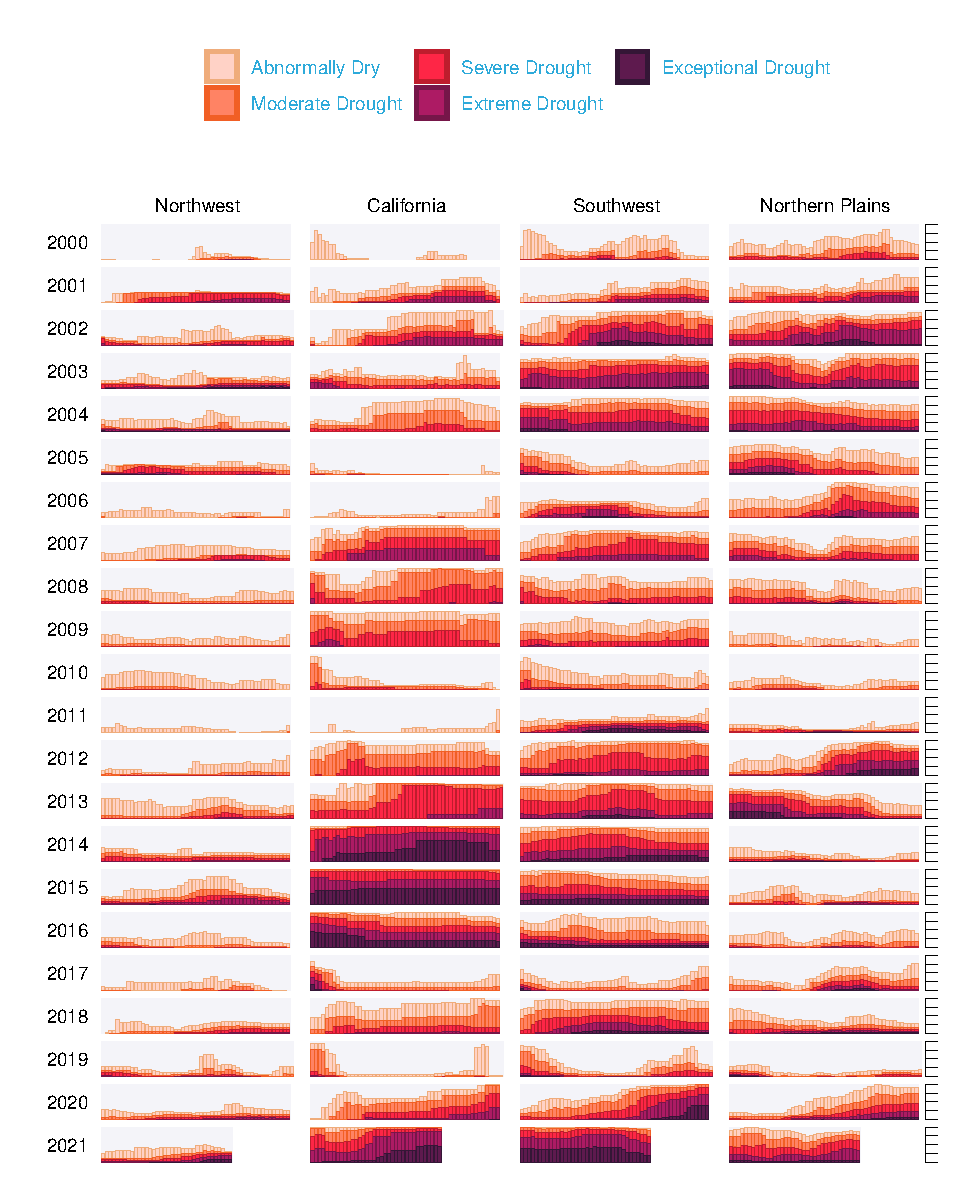
\includegraphics[width=1\linewidth]{data-viz_files/figure-latex/unnamed-chunk-32-1}

Up to this point, we've focused on one of the single plots that make up the larger data viz.~But the final product that Cédric and Georgios made is actually 176 plots (22 years and 8 regions). One of the most useful features of ggplot is what's known as facetting (known more commonly in the data viz world as small multiples). With the \texttt{facet\_grid()} function, we can select which variable to put in rows and which to put in columns of our facetted plot. Cédric and Georgios put \texttt{year} in rows and \texttt{hub} (region) in columns. The \texttt{switch\ =\ "y"} argument moves the year label from the right side (where it appears by default) to the left. With this code in place, we can see the final plot coming together. Space considerations require me to again include only four regions, but you get the idea.

\begin{Shaded}
\begin{Highlighting}[]
\NormalTok{dm\_perc\_cat\_hubs }\SpecialCharTok{\%\textgreater{}\%}
  \FunctionTok{filter}\NormalTok{(hub }\SpecialCharTok{\%in\%} \FunctionTok{c}\NormalTok{(}\StringTok{"Northwest"}\NormalTok{, }
                    \StringTok{"California"}\NormalTok{, }
                    \StringTok{"Southwest"}\NormalTok{, }
                    \StringTok{"Northern Plains"}\NormalTok{)) }\SpecialCharTok{\%\textgreater{}\%}
  \FunctionTok{ggplot}\NormalTok{(}\FunctionTok{aes}\NormalTok{(}\AttributeTok{x =}\NormalTok{ week, }
             \AttributeTok{y =}\NormalTok{ percentage,}
             \AttributeTok{fill =}\NormalTok{ category)) }\SpecialCharTok{+}
  \FunctionTok{geom\_col}\NormalTok{() }\SpecialCharTok{+}
  \FunctionTok{scale\_fill\_viridis\_d}\NormalTok{(}
    \AttributeTok{option =} \StringTok{"rocket"}\NormalTok{,}
    \AttributeTok{direction =} \SpecialCharTok{{-}}\DecValTok{1}
\NormalTok{  ) }\SpecialCharTok{+}
  \FunctionTok{scale\_x\_continuous}\NormalTok{(}\AttributeTok{name =} \ConstantTok{NULL}\NormalTok{, }
                     \AttributeTok{guide =} \StringTok{"none"}\NormalTok{) }\SpecialCharTok{+}
  \FunctionTok{scale\_y\_continuous}\NormalTok{(}\AttributeTok{name =} \ConstantTok{NULL}\NormalTok{, }
                     \AttributeTok{labels =} \ConstantTok{NULL}\NormalTok{, }
                     \AttributeTok{position =} \StringTok{"right"}\NormalTok{) }\SpecialCharTok{+}
  \FunctionTok{facet\_grid}\NormalTok{(}\AttributeTok{rows =} \FunctionTok{vars}\NormalTok{(year), }
             \AttributeTok{cols =} \FunctionTok{vars}\NormalTok{(hub), }
             \AttributeTok{switch =} \StringTok{"y"}\NormalTok{)}
\end{Highlighting}
\end{Shaded}

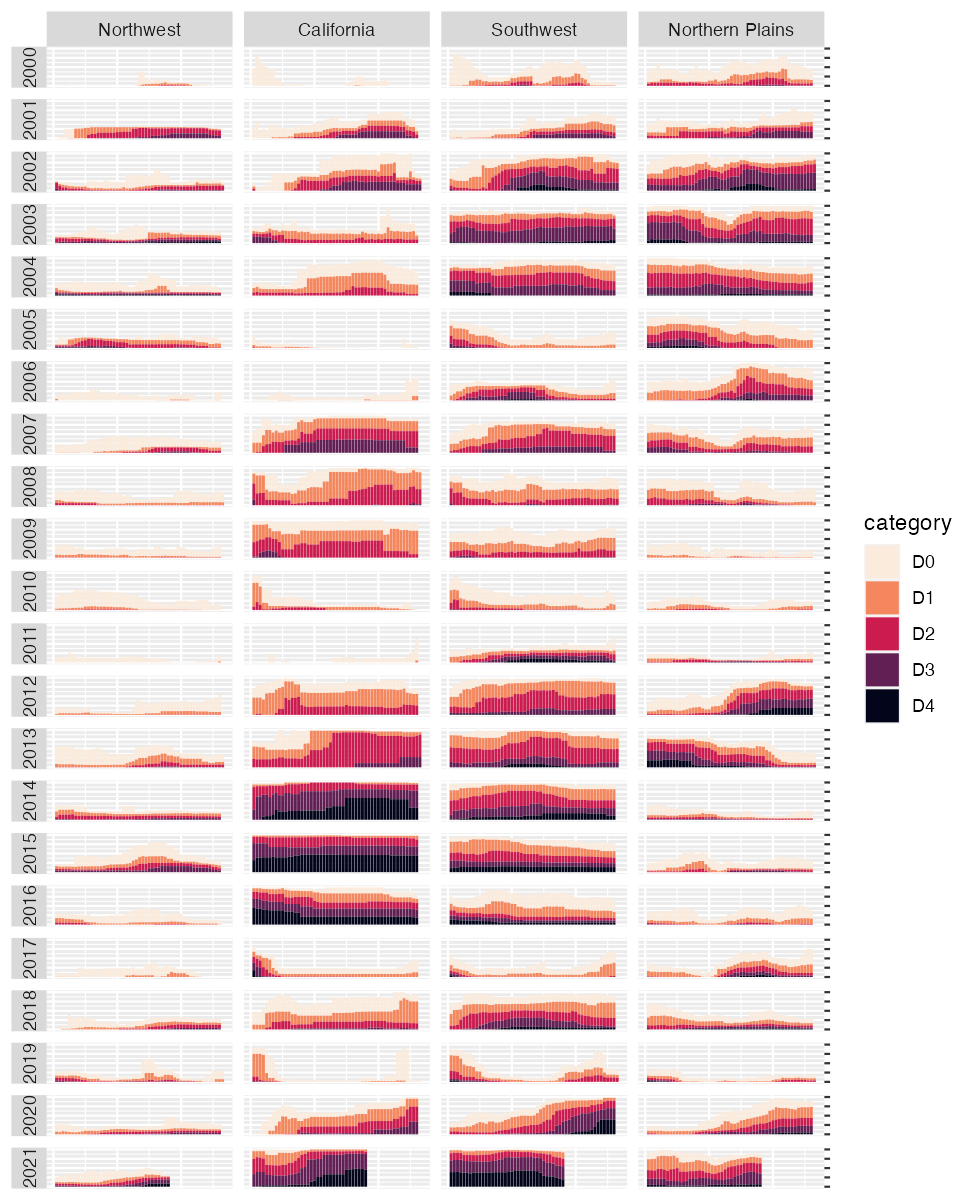
\includegraphics[width=1\linewidth]{data-viz_files/figure-latex/unnamed-chunk-34-1}

Incredibly, the broad outlines of the plot took us just 10 lines to create. All of the final code from here on out falls in the category of small polishes. That's not to minimize how important small polishes are (very) or the time it takes to create them (lots). But it is to say that a little bit of ggplot goes a long way.

Let's look at a few of the small polishes that Cédric and Georgios make. The first is to apply a theme. They use \texttt{theme\_light()}, which removes the default gray background and changes the font to Roboto.

\begin{Shaded}
\begin{Highlighting}[]
\NormalTok{dm\_perc\_cat\_hubs }\SpecialCharTok{\%\textgreater{}\%}
  \FunctionTok{filter}\NormalTok{(hub }\SpecialCharTok{\%in\%} \FunctionTok{c}\NormalTok{(}\StringTok{"Northwest"}\NormalTok{, }
                    \StringTok{"California"}\NormalTok{, }
                    \StringTok{"Southwest"}\NormalTok{, }
                    \StringTok{"Northern Plains"}\NormalTok{)) }\SpecialCharTok{\%\textgreater{}\%}
  \FunctionTok{ggplot}\NormalTok{(}\FunctionTok{aes}\NormalTok{(}\AttributeTok{x =}\NormalTok{ week, }
             \AttributeTok{y =}\NormalTok{ percentage,}
             \AttributeTok{fill =}\NormalTok{ category)) }\SpecialCharTok{+}
  \FunctionTok{geom\_col}\NormalTok{() }\SpecialCharTok{+}
  \FunctionTok{scale\_fill\_viridis\_d}\NormalTok{(}
    \AttributeTok{option =} \StringTok{"rocket"}\NormalTok{,}
    \AttributeTok{direction =} \SpecialCharTok{{-}}\DecValTok{1}
\NormalTok{  ) }\SpecialCharTok{+}
  \FunctionTok{scale\_x\_continuous}\NormalTok{(}\AttributeTok{name =} \ConstantTok{NULL}\NormalTok{, }
                     \AttributeTok{guide =} \StringTok{"none"}\NormalTok{) }\SpecialCharTok{+}
  \FunctionTok{scale\_y\_continuous}\NormalTok{(}\AttributeTok{name =} \ConstantTok{NULL}\NormalTok{, }
                     \AttributeTok{labels =} \ConstantTok{NULL}\NormalTok{, }
                     \AttributeTok{position =} \StringTok{"right"}\NormalTok{) }\SpecialCharTok{+}
  \FunctionTok{facet\_grid}\NormalTok{(}\AttributeTok{rows =} \FunctionTok{vars}\NormalTok{(year), }
             \AttributeTok{cols =} \FunctionTok{vars}\NormalTok{(hub), }
             \AttributeTok{switch =} \StringTok{"y"}\NormalTok{) }\SpecialCharTok{+}
  \FunctionTok{theme\_light}\NormalTok{(}\AttributeTok{base\_family =} \StringTok{"Roboto"}\NormalTok{)}
\end{Highlighting}
\end{Shaded}

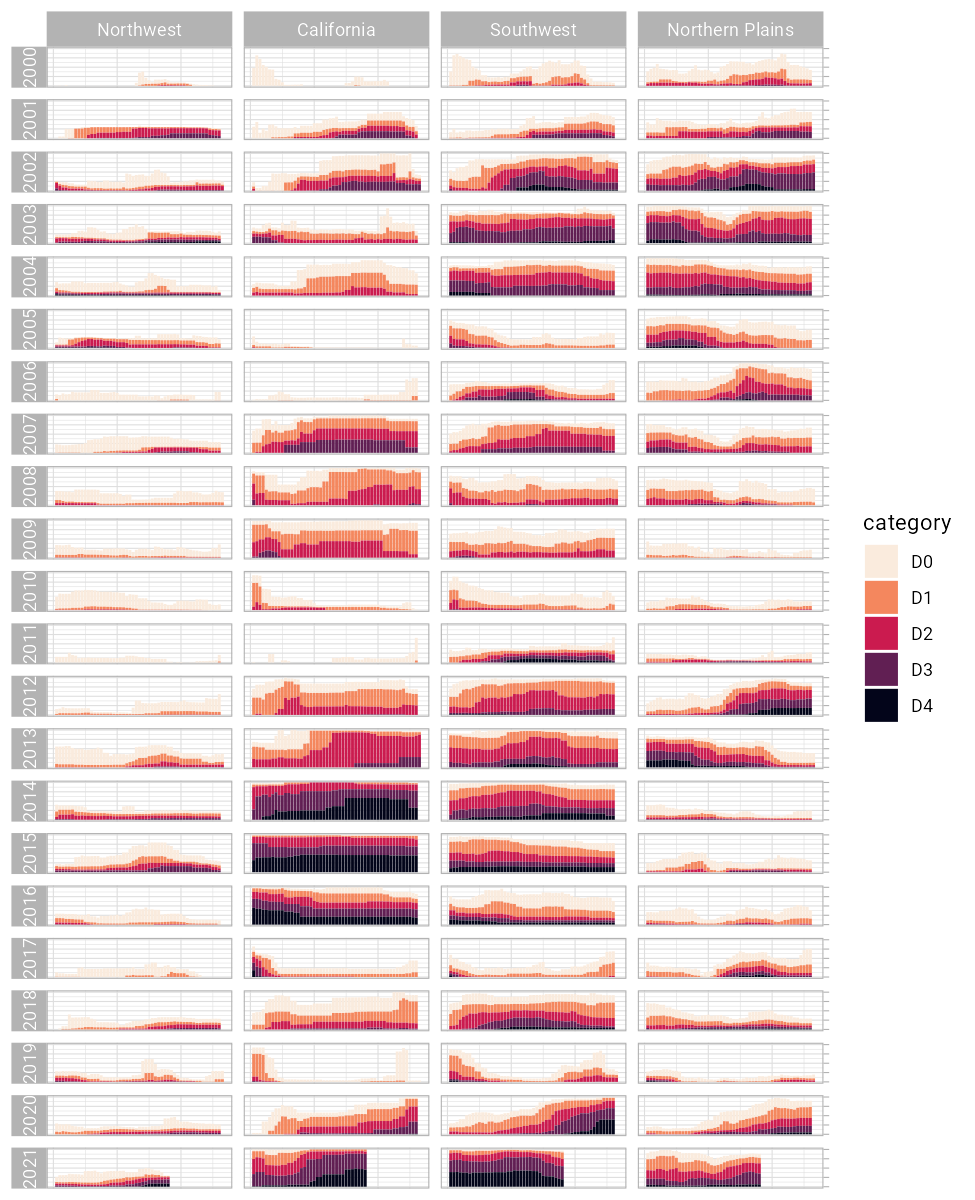
\includegraphics[width=1\linewidth]{data-viz_files/figure-latex/unnamed-chunk-36-1}

\texttt{theme\_light()} is what's known as a ``complete theme.'' So-called complete themes change the overall look-and-feel of a plot. But Cédric and Georgios don't stop with applying a complete theme. From there, they use the \texttt{theme()} function to make additional tweaks to what \texttt{theme\_light()} gives them.

\begin{Shaded}
\begin{Highlighting}[]
\NormalTok{dm\_perc\_cat\_hubs }\SpecialCharTok{\%\textgreater{}\%}
  \FunctionTok{filter}\NormalTok{(hub }\SpecialCharTok{\%in\%} \FunctionTok{c}\NormalTok{(}\StringTok{"Northwest"}\NormalTok{, }
                    \StringTok{"California"}\NormalTok{, }
                    \StringTok{"Southwest"}\NormalTok{, }
                    \StringTok{"Northern Plains"}\NormalTok{)) }\SpecialCharTok{\%\textgreater{}\%}
  \FunctionTok{ggplot}\NormalTok{(}\FunctionTok{aes}\NormalTok{(}\AttributeTok{x =}\NormalTok{ week, }
             \AttributeTok{y =}\NormalTok{ percentage,}
             \AttributeTok{fill =}\NormalTok{ category)) }\SpecialCharTok{+}
  \FunctionTok{geom\_col}\NormalTok{() }\SpecialCharTok{+}
  \FunctionTok{scale\_fill\_viridis\_d}\NormalTok{(}
    \AttributeTok{option =} \StringTok{"rocket"}\NormalTok{,}
    \AttributeTok{direction =} \SpecialCharTok{{-}}\DecValTok{1}
\NormalTok{  ) }\SpecialCharTok{+}
  \FunctionTok{scale\_x\_continuous}\NormalTok{(}\AttributeTok{name =} \ConstantTok{NULL}\NormalTok{, }
                     \AttributeTok{guide =} \StringTok{"none"}\NormalTok{) }\SpecialCharTok{+}
  \FunctionTok{scale\_y\_continuous}\NormalTok{(}\AttributeTok{name =} \ConstantTok{NULL}\NormalTok{, }
                     \AttributeTok{labels =} \ConstantTok{NULL}\NormalTok{, }
                     \AttributeTok{position =} \StringTok{"right"}\NormalTok{) }\SpecialCharTok{+}
  \FunctionTok{facet\_grid}\NormalTok{(}\AttributeTok{rows =} \FunctionTok{vars}\NormalTok{(year), }
             \AttributeTok{cols =} \FunctionTok{vars}\NormalTok{(hub), }
             \AttributeTok{switch =} \StringTok{"y"}\NormalTok{) }\SpecialCharTok{+}
  \FunctionTok{theme\_light}\NormalTok{(}\AttributeTok{base\_family =} \StringTok{"Roboto"}\NormalTok{) }\SpecialCharTok{+}
  \FunctionTok{theme}\NormalTok{(}
    \AttributeTok{axis.title =} \FunctionTok{element\_text}\NormalTok{(}\AttributeTok{size =} \DecValTok{14}\NormalTok{, }
                              \AttributeTok{color =} \StringTok{"black"}\NormalTok{),}
    \AttributeTok{axis.text =} \FunctionTok{element\_text}\NormalTok{(}\AttributeTok{family =} \StringTok{"Roboto Mono"}\NormalTok{, }
                             \AttributeTok{size =} \DecValTok{11}\NormalTok{),}
    \AttributeTok{axis.line.x =} \FunctionTok{element\_blank}\NormalTok{(),}
    \AttributeTok{axis.line.y =} \FunctionTok{element\_line}\NormalTok{(}\AttributeTok{color =} \StringTok{"black"}\NormalTok{, }
                               \AttributeTok{size =}\NormalTok{ .}\DecValTok{2}\NormalTok{),}
    \AttributeTok{axis.ticks.y =} \FunctionTok{element\_line}\NormalTok{(}\AttributeTok{color =} \StringTok{"black"}\NormalTok{, }
                                \AttributeTok{size =}\NormalTok{ .}\DecValTok{2}\NormalTok{),}
    \AttributeTok{axis.ticks.length.y =} \FunctionTok{unit}\NormalTok{(}\DecValTok{2}\NormalTok{, }\StringTok{"mm"}\NormalTok{),}
    \AttributeTok{legend.position =} \StringTok{"top"}\NormalTok{,}
    \AttributeTok{legend.title =} \FunctionTok{element\_text}\NormalTok{(}\AttributeTok{color =} \StringTok{"\#2DAADA"}\NormalTok{, }
                                \AttributeTok{face =} \StringTok{"bold"}\NormalTok{),}
    \AttributeTok{legend.text =} \FunctionTok{element\_text}\NormalTok{(}\AttributeTok{color =} \StringTok{"\#2DAADA"}\NormalTok{),}
    \AttributeTok{strip.text.x =} \FunctionTok{element\_text}\NormalTok{(}\AttributeTok{hjust =}\NormalTok{ .}\DecValTok{5}\NormalTok{, }
                                \AttributeTok{face =} \StringTok{"plain"}\NormalTok{, }
                                \AttributeTok{color =} \StringTok{"black"}\NormalTok{, }
                                \AttributeTok{margin =} \FunctionTok{margin}\NormalTok{(}\AttributeTok{t =} \DecValTok{20}\NormalTok{, }\AttributeTok{b =} \DecValTok{5}\NormalTok{)),}
    \AttributeTok{strip.text.y.left =} \FunctionTok{element\_text}\NormalTok{(}\AttributeTok{angle =} \DecValTok{0}\NormalTok{, }
                                     \AttributeTok{vjust =}\NormalTok{ .}\DecValTok{5}\NormalTok{, }
                                     \AttributeTok{face =} \StringTok{"plain"}\NormalTok{, }
                                     \AttributeTok{color =} \StringTok{"black"}\NormalTok{),}
    \AttributeTok{strip.background =} \FunctionTok{element\_rect}\NormalTok{(}\AttributeTok{fill =} \StringTok{"transparent"}\NormalTok{, }
                                    \AttributeTok{color =} \StringTok{"transparent"}\NormalTok{),}
    \AttributeTok{panel.grid.minor =} \FunctionTok{element\_blank}\NormalTok{(),}
    \AttributeTok{panel.grid.major =} \FunctionTok{element\_blank}\NormalTok{(),}
    \AttributeTok{panel.spacing.x =} \FunctionTok{unit}\NormalTok{(}\FloatTok{0.3}\NormalTok{, }\StringTok{"lines"}\NormalTok{),}
    \AttributeTok{panel.spacing.y =} \FunctionTok{unit}\NormalTok{(}\FloatTok{0.25}\NormalTok{, }\StringTok{"lines"}\NormalTok{),}
    \AttributeTok{panel.background =} \FunctionTok{element\_rect}\NormalTok{(}\AttributeTok{fill =} \StringTok{"transparent"}\NormalTok{, }
                                    \AttributeTok{color =} \StringTok{"transparent"}\NormalTok{),}
    \AttributeTok{panel.border =} \FunctionTok{element\_rect}\NormalTok{(}\AttributeTok{color =} \StringTok{"transparent"}\NormalTok{, }
                                \AttributeTok{size =} \DecValTok{0}\NormalTok{),}
    \AttributeTok{plot.background =} \FunctionTok{element\_rect}\NormalTok{(}\AttributeTok{fill =} \StringTok{"transparent"}\NormalTok{, }
                                   \AttributeTok{color =} \StringTok{"transparent"}\NormalTok{, }
                                   \AttributeTok{size =}\NormalTok{ .}\DecValTok{4}\NormalTok{),}
    \AttributeTok{plot.margin =} \FunctionTok{margin}\NormalTok{(}\FunctionTok{rep}\NormalTok{(}\DecValTok{18}\NormalTok{, }\DecValTok{4}\NormalTok{))}
\NormalTok{  )}
\end{Highlighting}
\end{Shaded}

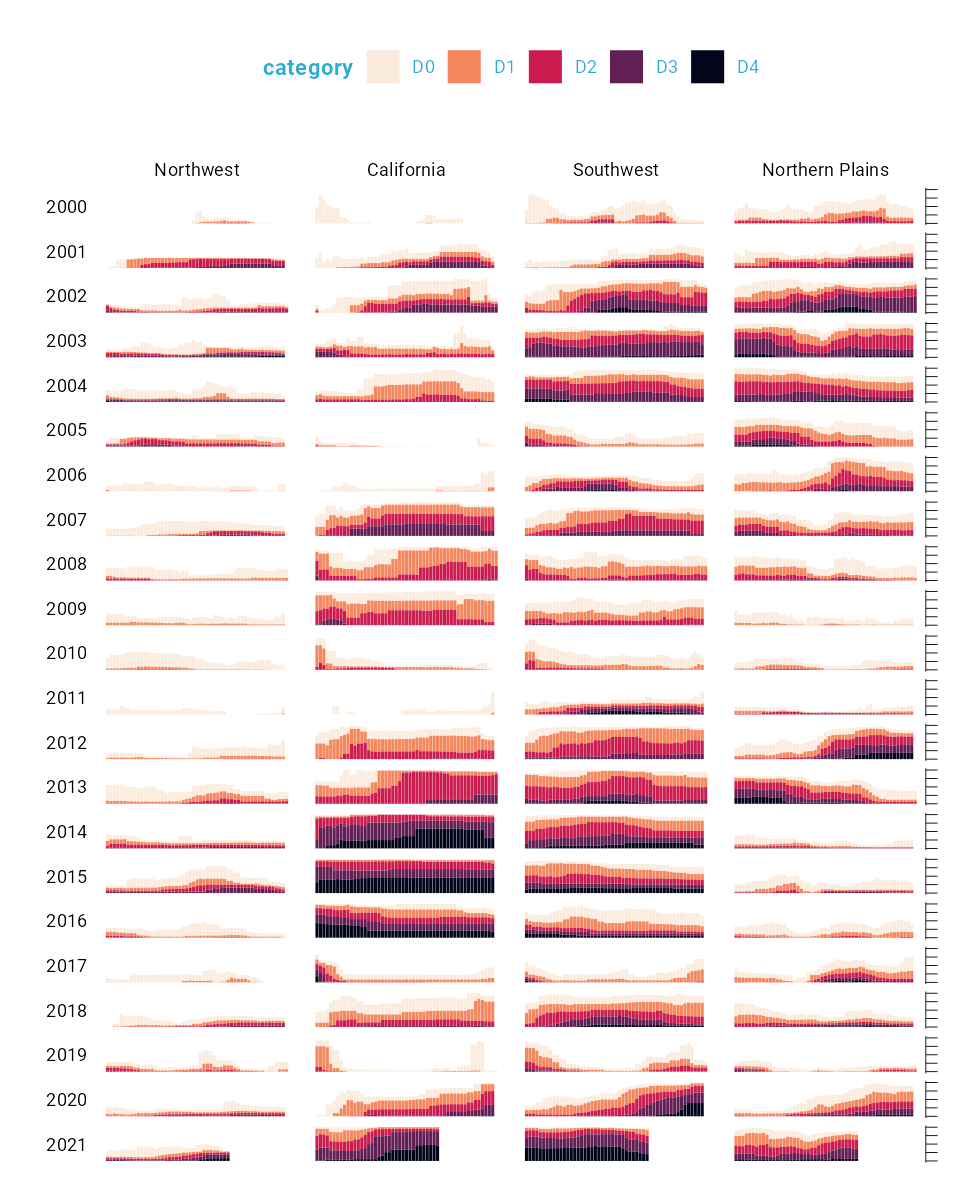
\includegraphics[width=1\linewidth]{data-viz_files/figure-latex/unnamed-chunk-38-1}

The code in the \texttt{theme()} function does many different things, but let's take a look at a few of the most important:

\texttt{legend.position\ =\ "top"} moves the legend from the right (the default) to the top of the plot.

\texttt{strip.text.y.left\ =\ element\_text(size\ =\ 18,\ angle\ =\ 0,\ vjust\ =\ .5,\ face\ =\ "plain",\ color\ =\ "black")} turns the year text in the columns so that it is no longer angled. Without the \texttt{angle\ =\ 0}, the years would be much less readable.

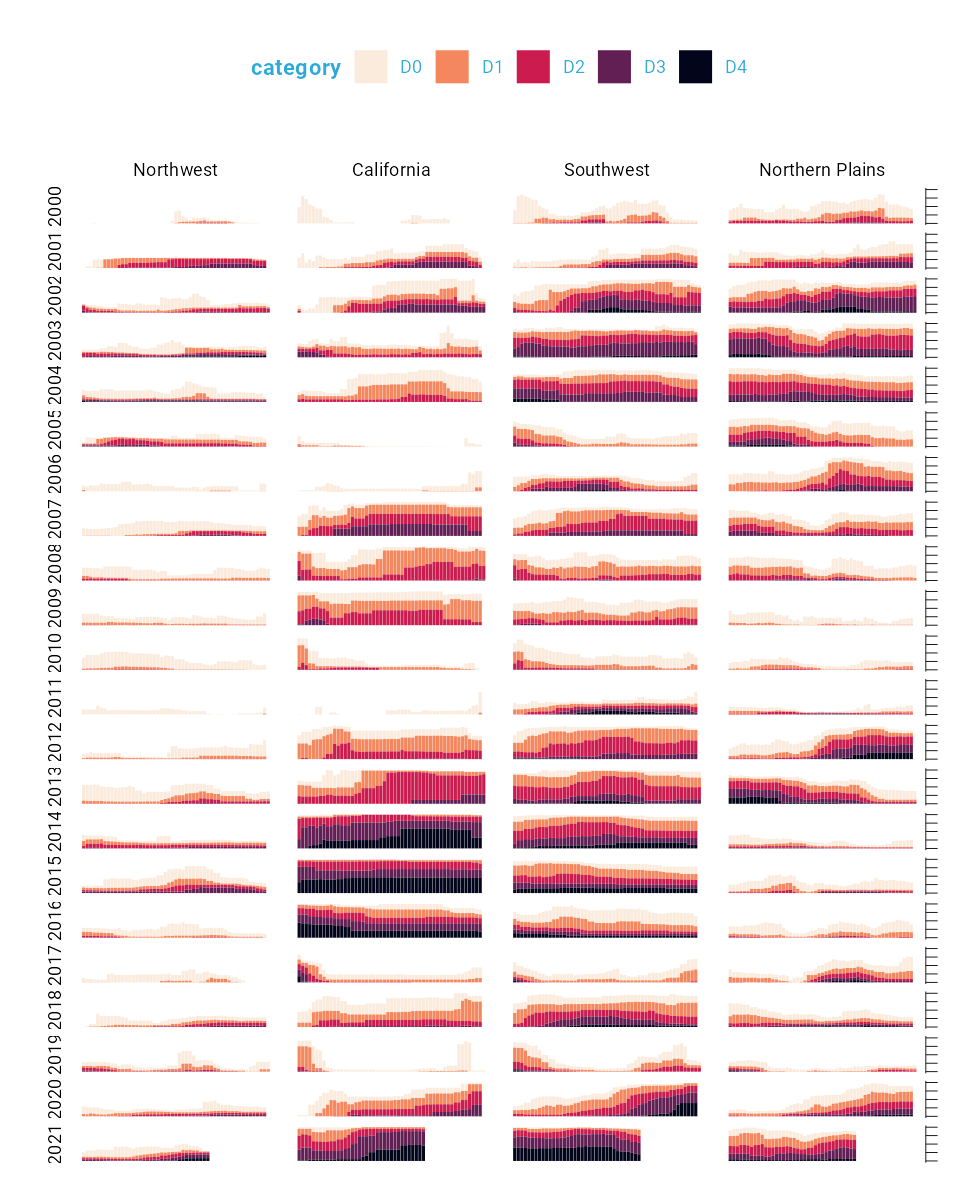
\includegraphics[width=1\linewidth]{data-viz_files/figure-latex/unnamed-chunk-40-1}

The following lines make the distinctive axis lines and ticks that show up on the right side of the final plot:

\begin{Shaded}
\begin{Highlighting}[]
\NormalTok{axis.line.x }\OtherTok{=} \FunctionTok{element\_blank}\NormalTok{(),}
\NormalTok{axis.line.y }\OtherTok{=} \FunctionTok{element\_line}\NormalTok{(}\AttributeTok{color =} \StringTok{"black"}\NormalTok{, }\AttributeTok{size =}\NormalTok{ .}\DecValTok{2}\NormalTok{),}
\NormalTok{axis.ticks.y }\OtherTok{=} \FunctionTok{element\_line}\NormalTok{(}\AttributeTok{color =} \StringTok{"black"}\NormalTok{, }\AttributeTok{size =}\NormalTok{ .}\DecValTok{2}\NormalTok{),}
\NormalTok{axis.ticks.length.y }\OtherTok{=} \FunctionTok{unit}\NormalTok{(}\DecValTok{2}\NormalTok{, }\StringTok{"mm"}\NormalTok{)}
\end{Highlighting}
\end{Shaded}

\texttt{panel.grid.minor\ =\ element\_blank()} and \texttt{panel.grid.major\ =\ element\_blank()} remove all grid lines from the final plot.

And finally, these three lines remove the borders and make each of the individual plots have a transparent background.

\begin{Shaded}
\begin{Highlighting}[]
\NormalTok{panel.background }\OtherTok{=} \FunctionTok{element\_rect}\NormalTok{(}\AttributeTok{fill =} \StringTok{"transparent"}\NormalTok{, }\AttributeTok{color =} \StringTok{"transparent"}\NormalTok{),}
\NormalTok{panel.border }\OtherTok{=} \FunctionTok{element\_rect}\NormalTok{(}\AttributeTok{color =} \StringTok{"transparent"}\NormalTok{, }\AttributeTok{size =} \DecValTok{0}\NormalTok{),}
\NormalTok{plot.background }\OtherTok{=} \FunctionTok{element\_rect}\NormalTok{(}\AttributeTok{fill =} \StringTok{"transparent"}\NormalTok{, }\AttributeTok{color =} \StringTok{"transparent"}\NormalTok{, }\AttributeTok{size =}\NormalTok{ .}\DecValTok{4}\NormalTok{)}
\end{Highlighting}
\end{Shaded}

Keen readers such as yourself may now be thinking: ``wait, didn't the individual plots have a gray background behind them?'' Yes, dear reader, they did. How did Cédric and Georgios make these? They did this with a separate geom: \texttt{geom\_rect()}. Here, they set some additional aesthetic properties specific to \texttt{geom\_rect()} (\texttt{xmin}, \texttt{xmax}, \texttt{ymin}, and \texttt{ymax}). The result is a gray background drawn behind each small multiple.

\begin{Shaded}
\begin{Highlighting}[]
\FunctionTok{geom\_rect}\NormalTok{(}
  \FunctionTok{aes}\NormalTok{(}
    \AttributeTok{xmin =}\NormalTok{ .}\DecValTok{5}\NormalTok{,}
    \AttributeTok{xmax =}\NormalTok{ max\_week }\SpecialCharTok{+}\NormalTok{ .}\DecValTok{5}\NormalTok{,}
    \AttributeTok{ymin =} \SpecialCharTok{{-}}\FloatTok{0.005}\NormalTok{,}
    \AttributeTok{ymax =} \DecValTok{1}
\NormalTok{  ),}
  \AttributeTok{fill =} \StringTok{"\#f4f4f9"}\NormalTok{,}
  \AttributeTok{color =} \ConstantTok{NA}\NormalTok{,}
  \AttributeTok{size =} \FloatTok{0.4}
\NormalTok{)}
\end{Highlighting}
\end{Shaded}

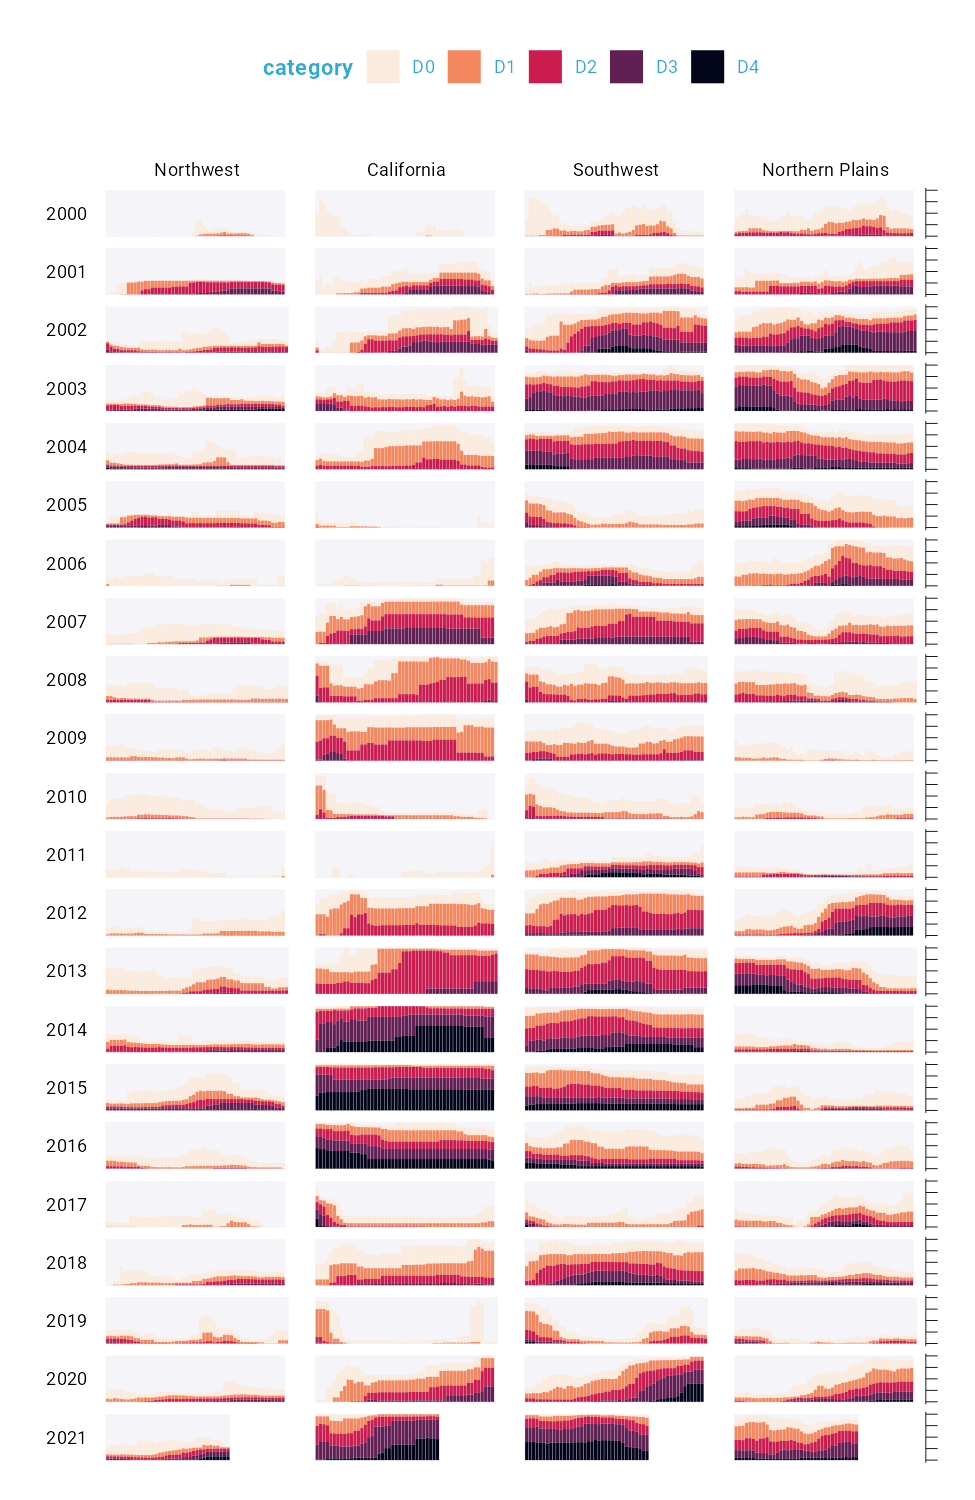
\includegraphics[width=1\linewidth]{data-viz_files/figure-latex/unnamed-chunk-45-1}

The final polish to highlight is the tweaks to the legend. I previously showed a simplified version of the \texttt{scale\_fill\_viridis\_d()} function. A more complete version is as follows. The \texttt{name} argument sets the legend title and the \texttt{labels} argument determine the labels that show up in the legend. Rather than D0, D1, D2, D3, and D4, we now have Abnormally Dry, Moderate Drought, Severe Drought, Extreme Drought, and Exceptional Drought.

\begin{Shaded}
\begin{Highlighting}[]
\FunctionTok{scale\_fill\_viridis\_d}\NormalTok{(}
  \AttributeTok{option =} \StringTok{"rocket"}\NormalTok{,}
  \AttributeTok{direction =} \SpecialCharTok{{-}}\DecValTok{1}\NormalTok{,}
  \AttributeTok{name =} \StringTok{"Category:"}\NormalTok{,}
  \AttributeTok{labels =} \FunctionTok{c}\NormalTok{(}
    \StringTok{"Abnormally Dry"}\NormalTok{,}
    \StringTok{"Moderate Drought"}\NormalTok{,}
    \StringTok{"Severe Drought"}\NormalTok{,}
    \StringTok{"Extreme Drought"}\NormalTok{,}
    \StringTok{"Exceptional Drought"}
\NormalTok{  )}
\NormalTok{)}
\end{Highlighting}
\end{Shaded}

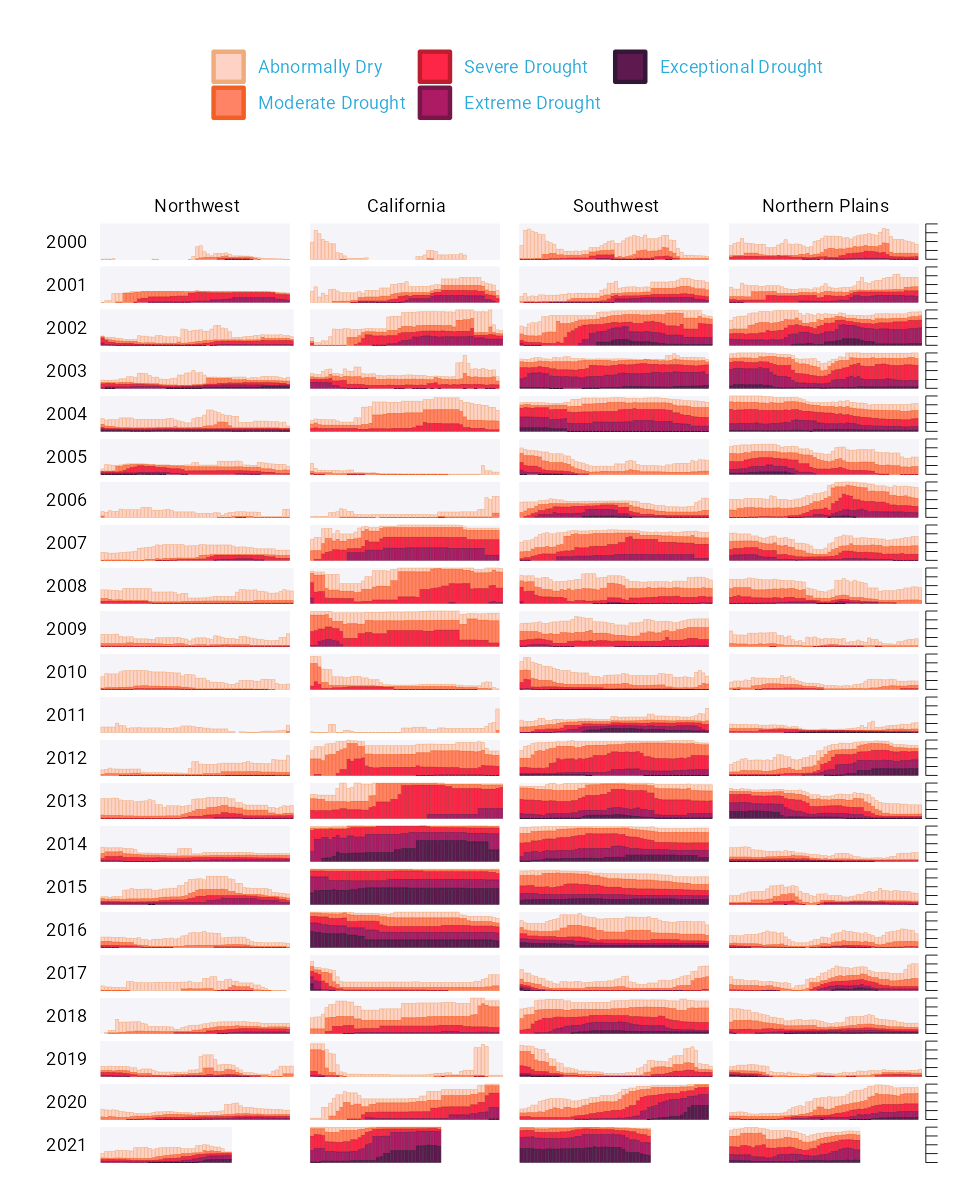
\includegraphics[width=1\linewidth]{data-viz_files/figure-latex/unnamed-chunk-48-1}

While I've showed you a nearly complete version of the code, I have made some small changes along the way to make it easier to understand. If you're curious to see the full code Cédric and Georgios used to create the data viz, here it is. There are a few additional tweaks to colors and spacing, but nothing major beyond what we've seen so far.

\begin{Shaded}
\begin{Highlighting}[]
\FunctionTok{ggplot}\NormalTok{(dm\_perc\_cat\_hubs, }\FunctionTok{aes}\NormalTok{(week, percentage)) }\SpecialCharTok{+}
  \FunctionTok{geom\_rect}\NormalTok{(}
    \FunctionTok{aes}\NormalTok{(}
      \AttributeTok{xmin =}\NormalTok{ .}\DecValTok{5}\NormalTok{,}
      \AttributeTok{xmax =}\NormalTok{ max\_week }\SpecialCharTok{+}\NormalTok{ .}\DecValTok{5}\NormalTok{,}
      \AttributeTok{ymin =} \SpecialCharTok{{-}}\FloatTok{0.005}\NormalTok{,}
      \AttributeTok{ymax =} \DecValTok{1}
\NormalTok{    ),}
    \AttributeTok{fill =} \StringTok{"\#f4f4f9"}\NormalTok{,}
    \AttributeTok{color =} \ConstantTok{NA}\NormalTok{,}
    \AttributeTok{size =} \FloatTok{0.4}\NormalTok{,}
    \AttributeTok{show.legend =} \ConstantTok{FALSE}
\NormalTok{  ) }\SpecialCharTok{+}
  \FunctionTok{geom\_col}\NormalTok{(}
    \FunctionTok{aes}\NormalTok{(}
      \AttributeTok{fill =}\NormalTok{ category,}
      \AttributeTok{fill =} \FunctionTok{after\_scale}\NormalTok{(}\FunctionTok{addmix}\NormalTok{(}\FunctionTok{darken}\NormalTok{(fill, .}\DecValTok{05}\NormalTok{, }
                                       \AttributeTok{space =} \StringTok{"HLS"}\NormalTok{), }
                                \StringTok{"\#d8005a"}\NormalTok{, }
\NormalTok{                                .}\DecValTok{15}\NormalTok{)),}
      \AttributeTok{color =} \FunctionTok{after\_scale}\NormalTok{(}\FunctionTok{darken}\NormalTok{(fill, .}\DecValTok{2}\NormalTok{, }
                                 \AttributeTok{space =} \StringTok{"HLS"}\NormalTok{))}
\NormalTok{    ),}
    \AttributeTok{width =}\NormalTok{ .}\DecValTok{9}\NormalTok{,}
    \AttributeTok{size =} \FloatTok{0.12}
\NormalTok{  ) }\SpecialCharTok{+}
  \FunctionTok{facet\_grid}\NormalTok{(}\AttributeTok{rows =} \FunctionTok{vars}\NormalTok{(year), }
             \AttributeTok{cols =} \FunctionTok{vars}\NormalTok{(hub), }
             \AttributeTok{switch =} \StringTok{"y"}\NormalTok{) }\SpecialCharTok{+}
  \FunctionTok{coord\_cartesian}\NormalTok{(}\AttributeTok{clip =} \StringTok{"off"}\NormalTok{) }\SpecialCharTok{+}
  \FunctionTok{scale\_x\_continuous}\NormalTok{(}\AttributeTok{expand =} \FunctionTok{c}\NormalTok{(.}\DecValTok{02}\NormalTok{, .}\DecValTok{02}\NormalTok{), }
                     \AttributeTok{guide =} \StringTok{"none"}\NormalTok{, }
                     \AttributeTok{name =} \ConstantTok{NULL}\NormalTok{) }\SpecialCharTok{+}
  \FunctionTok{scale\_y\_continuous}\NormalTok{(}\AttributeTok{expand =} \FunctionTok{c}\NormalTok{(}\DecValTok{0}\NormalTok{, }\DecValTok{0}\NormalTok{), }
                     \AttributeTok{position =} \StringTok{"right"}\NormalTok{, }
                     \AttributeTok{labels =} \ConstantTok{NULL}\NormalTok{, }
                     \AttributeTok{name =} \ConstantTok{NULL}\NormalTok{) }\SpecialCharTok{+}
  \FunctionTok{scale\_fill\_viridis\_d}\NormalTok{(}
    \AttributeTok{option =} \StringTok{"rocket"}\NormalTok{,}
    \AttributeTok{name =} \StringTok{"Category:"}\NormalTok{,}
    \AttributeTok{direction =} \SpecialCharTok{{-}}\DecValTok{1}\NormalTok{,}
    \AttributeTok{begin =}\NormalTok{ .}\DecValTok{17}\NormalTok{,}
    \AttributeTok{end =}\NormalTok{ .}\DecValTok{97}\NormalTok{,}
    \AttributeTok{labels =} \FunctionTok{c}\NormalTok{(}
      \StringTok{"Abnormally Dry"}\NormalTok{,}
      \StringTok{"Moderate Drought"}\NormalTok{,}
      \StringTok{"Severe Drought"}\NormalTok{,}
      \StringTok{"Extreme Drought"}\NormalTok{,}
      \StringTok{"Exceptional Drought"}
\NormalTok{    )}
\NormalTok{  ) }\SpecialCharTok{+}
  \FunctionTok{guides}\NormalTok{(}\AttributeTok{fill =} \FunctionTok{guide\_legend}\NormalTok{(}\AttributeTok{nrow =} \DecValTok{2}\NormalTok{,}
                             \AttributeTok{override.aes =} \FunctionTok{list}\NormalTok{(}\AttributeTok{size =} \DecValTok{1}\NormalTok{))) }\SpecialCharTok{+}
  \FunctionTok{theme\_light}\NormalTok{(}\AttributeTok{base\_size =} \DecValTok{18}\NormalTok{, }
              \AttributeTok{base\_family =} \StringTok{"Roboto"}\NormalTok{) }\SpecialCharTok{+}
  \FunctionTok{theme}\NormalTok{(}
    \AttributeTok{axis.title =} \FunctionTok{element\_text}\NormalTok{(}\AttributeTok{size =} \DecValTok{14}\NormalTok{, }
                              \AttributeTok{color =} \StringTok{"black"}\NormalTok{),}
    \AttributeTok{axis.text =} \FunctionTok{element\_text}\NormalTok{(}\AttributeTok{family =} \StringTok{"Roboto Mono"}\NormalTok{, }
                             \AttributeTok{size =} \DecValTok{11}\NormalTok{),}
    \AttributeTok{axis.line.x =} \FunctionTok{element\_blank}\NormalTok{(),}
    \AttributeTok{axis.line.y =} \FunctionTok{element\_line}\NormalTok{(}\AttributeTok{color =} \StringTok{"black"}\NormalTok{, }
                               \AttributeTok{size =}\NormalTok{ .}\DecValTok{2}\NormalTok{),}
    \AttributeTok{axis.ticks.y =} \FunctionTok{element\_line}\NormalTok{(}\AttributeTok{color =} \StringTok{"black"}\NormalTok{, }
                                \AttributeTok{size =}\NormalTok{ .}\DecValTok{2}\NormalTok{),}
    \AttributeTok{axis.ticks.length.y =} \FunctionTok{unit}\NormalTok{(}\DecValTok{2}\NormalTok{, }\StringTok{"mm"}\NormalTok{),}
    \AttributeTok{legend.position =} \StringTok{"top"}\NormalTok{,}
    \AttributeTok{legend.title =} \FunctionTok{element\_text}\NormalTok{(}\AttributeTok{color =} \StringTok{"\#2DAADA"}\NormalTok{, }
                                \AttributeTok{size =} \DecValTok{18}\NormalTok{, }
                                \AttributeTok{face =} \StringTok{"bold"}\NormalTok{),}
    \AttributeTok{legend.text =} \FunctionTok{element\_text}\NormalTok{(}\AttributeTok{color =} \StringTok{"\#2DAADA"}\NormalTok{, }
                               \AttributeTok{size =} \DecValTok{16}\NormalTok{),}
    \AttributeTok{strip.text.x =} \FunctionTok{element\_text}\NormalTok{(}\AttributeTok{size =} \DecValTok{16}\NormalTok{, }
                                \AttributeTok{hjust =}\NormalTok{ .}\DecValTok{5}\NormalTok{, }
                                \AttributeTok{face =} \StringTok{"plain"}\NormalTok{, }
                                \AttributeTok{color =} \StringTok{"black"}\NormalTok{, }
                                \AttributeTok{margin =} \FunctionTok{margin}\NormalTok{(}\AttributeTok{t =} \DecValTok{20}\NormalTok{, }\AttributeTok{b =} \DecValTok{5}\NormalTok{)),}
    \AttributeTok{strip.text.y.left =} \FunctionTok{element\_text}\NormalTok{(}\AttributeTok{size =} \DecValTok{18}\NormalTok{, }
                                     \AttributeTok{angle =} \DecValTok{0}\NormalTok{, }
                                     \AttributeTok{vjust =}\NormalTok{ .}\DecValTok{5}\NormalTok{, }
                                     \AttributeTok{face =} \StringTok{"plain"}\NormalTok{, }
                                     \AttributeTok{color =} \StringTok{"black"}\NormalTok{),}
    \AttributeTok{strip.background =} \FunctionTok{element\_rect}\NormalTok{(}\AttributeTok{fill =} \StringTok{"transparent"}\NormalTok{, }
                                    \AttributeTok{color =} \StringTok{"transparent"}\NormalTok{),}
    \AttributeTok{panel.grid.minor =} \FunctionTok{element\_blank}\NormalTok{(),}
    \AttributeTok{panel.grid.major =} \FunctionTok{element\_blank}\NormalTok{(),}
    \AttributeTok{panel.spacing.x =} \FunctionTok{unit}\NormalTok{(}\FloatTok{0.3}\NormalTok{, }\StringTok{"lines"}\NormalTok{),}
    \AttributeTok{panel.spacing.y =} \FunctionTok{unit}\NormalTok{(}\FloatTok{0.25}\NormalTok{, }\StringTok{"lines"}\NormalTok{),}
    \AttributeTok{panel.background =} \FunctionTok{element\_rect}\NormalTok{(}\AttributeTok{fill =} \StringTok{"transparent"}\NormalTok{, }
                                    \AttributeTok{color =} \StringTok{"transparent"}\NormalTok{),}
    \AttributeTok{panel.border =} \FunctionTok{element\_rect}\NormalTok{(}\AttributeTok{color =} \StringTok{"transparent"}\NormalTok{, }
                                \AttributeTok{size =} \DecValTok{0}\NormalTok{),}
    \AttributeTok{plot.background =} \FunctionTok{element\_rect}\NormalTok{(}\AttributeTok{fill =} \StringTok{"transparent"}\NormalTok{, }
                                   \AttributeTok{color =} \StringTok{"transparent"}\NormalTok{, }
                                   \AttributeTok{size =}\NormalTok{ .}\DecValTok{4}\NormalTok{),}
    \AttributeTok{plot.margin =} \FunctionTok{margin}\NormalTok{(}\FunctionTok{rep}\NormalTok{(}\DecValTok{18}\NormalTok{, }\DecValTok{4}\NormalTok{))}
\NormalTok{  )}
\end{Highlighting}
\end{Shaded}

\hypertarget{ggplot-is-your-data-viz-secret-weapon}{%
\section{ggplot is Your Data Viz Secret Weapon}\label{ggplot-is-your-data-viz-secret-weapon}}

If you take up ggplot, you may start to think of it as a solution to all of your data viz problems. Yes, you have a new hammer, but no, everything is not a nail. If you look at the version of this data viz that appeared in Scientific American\footnote{\url{https://www.scientificamerican.com/article/climate-change-drives-escalating-drought/}}, you'll see that there are some annotations not visible in our recreation. That's because they were added in post-production outside of ggplot. While you \emph{can} come up with ways to do everything in ggplot, it's often not the best use of your time. Get yourself 90\% of the way there with ggplot and then use Illustrator, Figma, or a similar tool to finish off your work.

With that caveat in place, ggplot is a very powerful hammer. And it's a hammer used to make plots that you've seen in the New York Times, FiveThirtyEight, the BBC, and other well-known news outlets. ggplot is so popular not because it is the only tool that can make data viz that follows principles of high-quality data viz, but because it makes it straightforward to do so. The graph that Cédric Scherer and Georgios Karamanis made shows this in several ways:

\begin{enumerate}
\def\labelenumi{\arabic{enumi}.}
\tightlist
\item
  \textbf{It strips away extraneous elements such as grid lines in order to keep the focus on the data itself}. Complete themes such as \texttt{theme\_light()} and the \texttt{theme()} function allowed Cédric and Georgios to create a decluttered visualization that communicates effectively.
\item
  \textbf{It uses well-chosen colors}. The \texttt{scale\_fill\_viridis\_d()} allowed them to create a color scheme that shows differences between groups well, is both colorblind-friendly, and shows up well when printed in grayscale.
\item
  \textbf{It uses small multiples to break data from two decades and eight regions into a set of graphs that come together to create a single plot.} With a single call to the \texttt{facet\_grid()} function, Cédric and Georgios created over 100 small multiples that are automatically combined into a single plot.
\end{enumerate}

Learning to create data visualization in ggplot involves a significant time investment. But the long-term payoff is even greater. Once you learn how ggplot works, you can look at others' code and learn how to improve your own. Take Cédric and Georgios's code, run it on your own system, and the beautiful visualization they made will magically appear.\\
Being able to run and learn from others' code is not something you can do in Excel. When you make a data viz in Excel, the series of point-and-click steps disappear into the ether with each use. Want to recreate a visualization you made last week? You'll need to remember the exact steps you used. Want to make a data viz that you saw someone else make? You'll need them to write up their process for you.

Code-based data viz tools like ggplot allow you to keep that record of the steps you made. In the end, that's all code is: a set of instructions. And it's a set of instructions that you can re-run or you can share with others for them to run. Or the reverse: others can share their code and you can learn from them. You don't have to be the most talented designer to make high-quality data viz with ggplot. You can study others' code, adapt it to your own needs, and create your own data viz with ggplot that is beautiful and communicates effectively.

\hypertarget{develop-a-custom-theme-to-keep-your-data-viz-consistent}{%
\chapter{Develop a Custom Theme to Keep Your Data Viz Consistent}\label{develop-a-custom-theme-to-keep-your-data-viz-consistent}}

\hypertarget{r-is-a-full-fledged-map-making-tool}{%
\chapter{R is a Full-Fledged Map-Making Tool}\label{r-is-a-full-fledged-map-making-tool}}

\hypertarget{make-tables-that-look-good-and-share-results-effectively}{%
\chapter{Make Tables That Look Good and Share Results Effectively}\label{make-tables-that-look-good-and-share-results-effectively}}

\url{https://clauswilke.com/dataviz/figure-titles-captions.html\#tables}

\hypertarget{part-communicate}{%
\chapter{(PART*) Communicate}\label{part-communicate}}

\hypertarget{use-rmarkdown-to-communicate-accurately-and-efficiently}{%
\chapter{Use RMarkdown to Communicate Accurately and Efficiently}\label{use-rmarkdown-to-communicate-accurately-and-efficiently}}

\hypertarget{use-rmarkdown-to-instantly-generate-hundreds-of-reports}{%
\chapter{Use RMarkdown to Instantly Generate Hundreds of Reports}\label{use-rmarkdown-to-instantly-generate-hundreds-of-reports}}

\hypertarget{create-beautiful-presentations-with-rmarkdown}{%
\chapter{Create Beautiful Presentations with RMarkdown}\label{create-beautiful-presentations-with-rmarkdown}}

\hypertarget{make-websites-to-share-results-online}{%
\chapter{Make Websites to Share Results Online}\label{make-websites-to-share-results-online}}

\begin{itemize}
\tightlist
\item
  When to do static vs when you need Shiny
\end{itemize}

\hypertarget{part-automate}{%
\chapter{(PART*) Automate}\label{part-automate}}

\hypertarget{access-up-to-date-census-data-with-the-tidycensus-package}{%
\chapter{\texorpdfstring{Access Up to Date Census Data with the \texttt{tidycensus} Package}{Access Up to Date Census Data with the tidycensus Package}}\label{access-up-to-date-census-data-with-the-tidycensus-package}}

\hypertarget{pull-in-survey-results-as-soon-as-they-come-in}{%
\chapter{Pull in Survey Results as Soon as They Come In}\label{pull-in-survey-results-as-soon-as-they-come-in}}

\hypertarget{stop-copying-and-pasting-code-by-creating-your-own-functions}{%
\chapter{Stop Copying and Pasting Code by Creating Your Own Functions}\label{stop-copying-and-pasting-code-by-creating-your-own-functions}}

\hypertarget{bundle-your-functions-together-in-your-own-r-package}{%
\chapter{Bundle Your Functions Together in Your Own R Package}\label{bundle-your-functions-together-in-your-own-r-package}}

\hypertarget{part-conclusion}{%
\chapter{(PART*) Conclusion}\label{part-conclusion}}

\hypertarget{come-for-the-data-stay-for-the-community}{%
\chapter{Come for the Data, Stay for the Community}\label{come-for-the-data-stay-for-the-community}}

\end{document}
